\documentclass[12pt]{report}
\usepackage{gensymb}
\usepackage{setspace}
\usepackage{caption}
\usepackage{subcaption}
\usepackage{breqn}
\usepackage{pgfplotstable}
\usepackage{array}
\usepackage{booktabs}
\usepackage{graphicx}
\usepackage{url}
\usepackage{fancyhdr}
\usepackage{siunitx}
\usepackage{hyperref}
\usepackage{natbib}
\hypersetup{
    colorlinks,
    citecolor=black,
    filecolor=black,
    linkcolor=black,
    urlcolor=black
}
\setlength{\parskip}{1em}
\graphicspath{ {images/} }
\setlength\headheight{20pt} 
\fancypagestyle{style1}{
  \fancyhf{}
  \cfoot{\thepage}
}
\fancypagestyle{title}{
\renewcommand{\headrulewidth}{0pt}
\chead{
\includegraphics[width=4cm]{rmit}}
}
\setcounter{secnumdepth}{3}
\begin{document}
\pagenumbering{Roman}
\pagestyle{title}
\title{
	{Detailed Analysis of the Relationship between Geometry and Airflow in Older Chinese Adult Male Nasal Cavities}\\
	{\large SAMME}\\
	{
\includegraphics{rmit.jpg}}
}
\author{Sean Read}

    \begin{center}
        

      \vspace*{1cm}
        
	Detailed Analysis of the Relationship between Geometry and Airflow in older Chinese Adult Male Nasal Cavities
        
        \vspace*{1cm}
        A thesis submitted in fulfilment of the requirements for the degree of Master’s by research
	\vspace{1.5cm}
        
        Sean Dermott Read
        
        \vspace{2.8cm}
        

        
	School of Aerospace Mechanical and Manufacturing Engineering\\
	\vspace{0.3cm}
        College of Science Engineering and Health\\
	\vspace{0.3cm}
	RMIT University\\
	\vspace{1cm}
	October 2016
        
    \end{center}
\onehalfspacing

 
\chapter*{Declaration}
\pagestyle{style1}
I certify that except where due acknowledgement has been made, the work is that of the author alone; the work has not been submitted previously, in whole or in part, to qualify for any other academic award; the content of the thesis is the result of work which has been carried out since the official commencement date of the approved research program; any editorial work, paid or unpaid, carried out by a third party is acknowledged; and, ethics procedures and guidelines have been followed\\


\vspace{0.3cm}
\noindent
Sean Dermott Read\\

\noindent
28th October 2016
\chapter*{Acknowledgements}
I want to thank my supervisors, Dr Kiao Inthavong and Professor Jiyuan Tu, my colleagues in the CFD group, my family and my partner Tao Yao. 

\tableofcontents

\newpage
\listoffigures
\listoftables

\chapter*{Abstract}
\pagenumbering{arabic}
\addcontentsline{toc}{chapter}{Abstract}
Older nasal cavities tend to exhibit a range of symptoms and pathologies more frequently than those of younger patients. These symptoms include variations in airconditioning functionality, as well as olfaction and mucosal clearance functionality. 
Several factors have been identified as potentially responsible for these symptoms. 
One issue that has been identified as a potential cause for a number of the identified symptoms is aberrations in airflow structures caused by age-related variations in nasal cavity anatomy. 
Various methods have been used to examine nasal patency between demographics, including Computational Fluid Dynamics (CFD) studies of airflow through nasal cavity models developed from Computed Tomography (CT) scans. 
To date CFD methods have not been used to examine airflow in older nasal cavities.
This study will apply previously developed techniques for interdemographic analysis to CFD simulation results from a series of older, Asian, adult male nasal cavity models.


Firstly the reconstruction methods used for creating the nasal cavity geometries are detailed.
The discretisation and setup of the CFD simulations carried out for the five models are then outlined.
The results are then discussed.


This study provides preliminary understanding connecting nasal anatomy, age and airflow dynamics. Although the study size was limited, it provides insight into potential relationships between inhaled airflow characteristics and geometry. In particular discrepencies are noted in pressure drop and wall shear distribution as well as heat and vapour transfer as a result of geometric variations between the models.


\chapter{Introduction}

\section{Background}

The ageing global population increases the need for investment in geriatrics. One area of particular significance within this field is that of rhinology. A range of dysfunctions and aberrations from the normal functioning of nasal cavities in healthy adults have been observed in the elderly population \cite{Edelstein1996, Lindemann2008}. For example, the occurrence of respiratory diseases in the elderly is markedly higher than that found in younger populations \cite{HO2001, Edelstein1996}. It has been suggested that these higher recorded rates could be due in part to the impaired air conditioning functionality \cite{Lindemann2008}.


The nasal cavities of elderly citizens exhibit increased volume \cite{Kalmovich2005}. Alterations in histiological function have also been shown \cite{HO2001}. The extent to which functional aberrations are caused by geometric (as opposed to histiological) variations remains unclear \cite{Varga-Huettner2013}. These changes in nasal physiology - and their impact on nasal functionality - need to be investigated further.


Computational Fluid Dynamics (CFD) numerically approximates flow field characteristics for a given domain. CFD simulations give highly detailed results with information covering a range of areas for a given fluid system at a minimal cost. One area in which CFD simulations have been gaining credence is that of biomechanics; many biological fluid systems can be modelled effectively through CFD simulations, allowing for an unprecedented insight into their function.

The use of 3D medical imaging techniques such as computed tomography (CT) scans in collaboration with CFD has facilitated the numerical approximation of fluid mechanism parameters in anatomically accurate models. This allows for more detailed analysis of the effects of topological variations on fluid mechanisms. This capacity for detailed comparison makes CFD simulation an ideal tool for analysing the impact of physiological discrepencies on nasal patency.


To date numerous inter-demographic studies have been carried out using CFD analysis of 3D models reconstructed from CT scan data \cite{Xi2012, Garcia2007, Zhu2011}. These studies have indicated that factors such as ethnicity and gender are liable to impact on nasal physiology. Previous studies have focused on age \cite{Xi2012}, however to date these age related studies have all focused on children. The use of CFD to examine functional variations in older models - accounting for potential interdemographic variations such as gender or ethnicity - is thus an important step that needs to be taken in order to achieve a more comprehensive understanding of the impact of ageing on nasal patency. For the sake of this thesis, the term older will be taken to mean ages of 60 and older.

\section{Literature review}
In this section the relevant literature regarding older nasal cavities will be reviewed. Significant gaps in the current body of knowledge will be identified and serve as the foundation for this thesis.

\subsection{Nasal cavity anatomy}


\begin{figure}
\centering
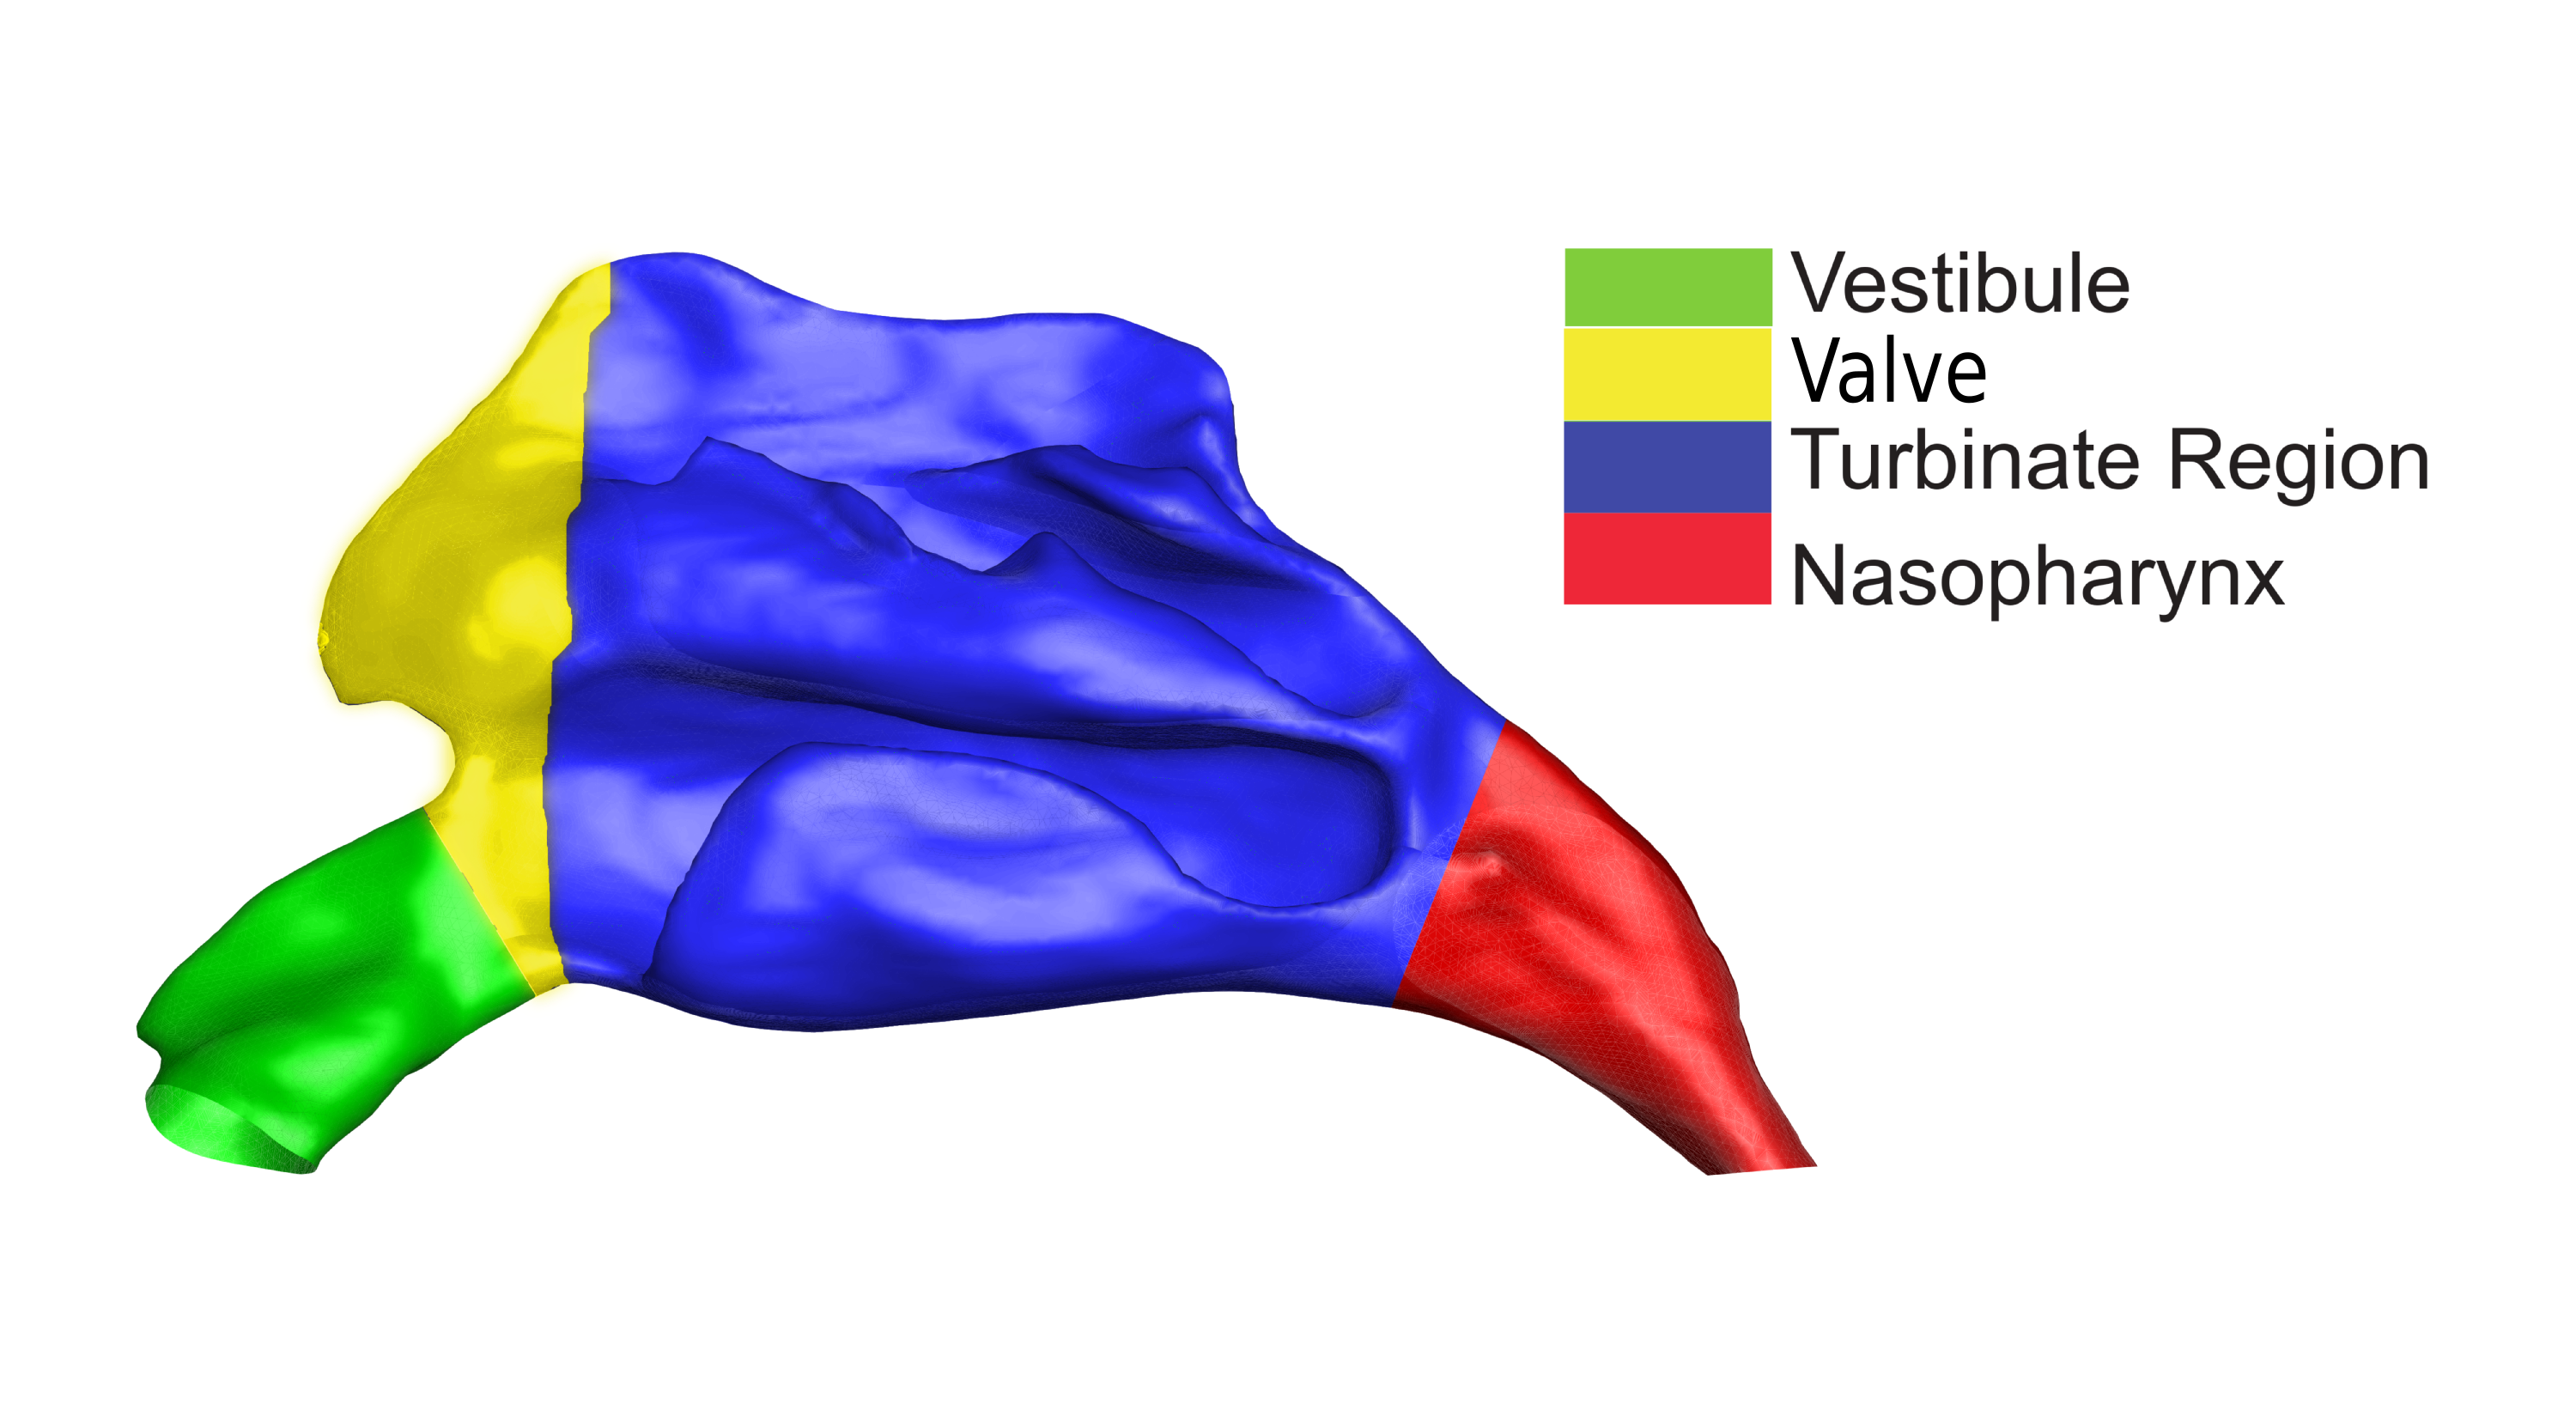
\includegraphics[width=0.7\textwidth]{regions}
\caption{Colour coded display of the anatomical regions of the nasal cavity} 
\label{fig:regions1}
\end{figure} 


The nasal cavity is the primary conduit for air coming into the respiratory system. \cite{Elad2008}. The nasal cavity consists of two 5 by 10 cm chambers running between the nostrils and the pharynx \cite{Mygind1998}. The cavities are each made up of three meatus. The meatus are connected to the nasolacrimal duct and paranasal sinuses, which are the largest of the many sinuses that surround the nasal cavity \cite{Mygind1998}. 
The nasal cavity is lined by respiratory epithelium. This epithelium controls the movement of mucous within the nasal cavity and is thus essential to its (the nasal cavity) airconditioning functionality \cite{Mygind1998}.
The two major functions of the nasal cavities are conditioning of the air for interaction with the internal airways by warming and humidification, and olfaction \cite{Doorly2008, Elad2008, Mygind1998, Berglund1982}.

\subsection{Geriatric rhinology}
Rhinology is the branch of medicine that deals with the nose and its pathologies. 
Common rhinological complaints of the elderly include dryness, runny noses, crusting and epistaxis \cite{Varga-Huettner2013}. Epidemiological studies have been carried out to examine the consistency of the manifestation of various symptoms throughout elderly patients with mixed results. 

The literature at present seems to be unanimous on the tendency of the nasal cavity's cross sectional area to increase with age. Several researchers have investigated this phenomena using acoustic rhinometry and shown good concordance in study outcomes \cite{Kalmovich2005, Edelstein1996,WhanKim2007,Lindemann2008}. Loftus et al. \cite{Loftus2016} compared the volumes of 22 nasal cavity models taken from CT scan data, and also found a clear tendency towards increased nasal cavity volume with ageing. Nasal air heating and humidification examined in vivo have been shown to be impaired in older patients; Lindemann et al. \cite{Lindemann2008} found average end-inspiratory temperature of $24^{\circ}C$ for older  patients as opposed to $27.1^{\circ}C$ for younger patients. Their findings for humidity were comparable. 

Increases in postnasal drip, nasal drainage, sneezing, coughing, olfactory dysfunction and gustatory rhinitis with age were observed in a clinical study of 131 patients \cite{Edelstein1996}. A 2009 study found that in a sample of 80 people no significant relationship could be observed between age and nasal discomfort \cite{Lindemann2010}. The same study, however, concurred with previous results on the increase of volume and cross sectional area as a function of age. Changes within the nose appear to not be limited to the increased volume; Both functional and structural variations in the respiratory epithelium have been observed with age, contributing to slower clearing of mucous \cite{HO2001}. 

Functional variations in air conditioning capabilities have been shown in vivo \cite{Lindemann2008}, with statistically significant reductions in relative humidity and heat transfer observed in elder nasal cavities. The level to which this is attributable to change in histological function as opposed to variations in the fluid mechanisms as a result of the expansion of the cavity remains to be investigated.

 \subsection{Experimental studies in rhinology}
 
To investigate air flow mechanisms in older nasal cavities, an experimental technique for the investigation must first be chosen. In this section the methods available for investigating nasal patency are presented.

The anatomy of the nasal cavity was first classified in detail by Emil Zuckerlandl in the 19th century \cite{Stammberger1989}. Anatomically, his records were more or less up to the standard of what can be assessed from modern scanning techniques \cite{Stammberger1989}, however the investigation of airflow characteristics was still severely limited by technological capacity \cite{Eccles2000}. It was not until the turn of the 19th century that experimentation in to nasal airflow began in proper \cite{Eccles2000}. 

Some of the more common in vivo techniques used include rhinomanometry, which measures of the pressure drop across the nasal cavity \cite{Hilberg1989}; and acoustic rhinometry, which allows measurement of the cross sectional area of the nasal cavity as a function of depth \cite{Hilberg1989}. 

Ultimately, however, direct detailed measurements of flow mechanics within the human nasal cavity taken in vivo are not practically viable with current technology as a result of the complexity and small scale of the nasal geometry \cite{Doorly2008c}. Thus the preferred media for the testing in modern times has tended to be either physical or computational models reconstructed from CT scan data \cite{Doorly2008c}. The physical models that have been constructed from CT scan data are able to provide detailed geometric reproductions.
These geometries can then be used to create accurate 3D models which can then be used with techniques like particle image velocimetry to conduct in detailed flow analysis throughout the nasal cavity \cite{Chung2008, Kelly2000}.
These techniques allow for data about instantaneous velocities at many points throughout a working fluid to be obtained through photographic methods. From this data the flow regime can be computed with high accuracy, allowing for in depth quantitave and qualitative analysis. Spence et al. \cite{Spence2012}, for example, showed detailed velocity contours from unsteady flow experiments using PIV.
Such experimental set ups are, however, costly to run in terms of time and resources, in particular when compared with the high level of detail that can be achieved from a well done CFD simulation \cite{Ma2009}.


\subsection{Computational studies}  
\subsubsection*{Background}
Computational fluid dynamics(CFD) is a discipline which is concerned with the computational approximation of solutions to the navier stokes equations for closed fluid systems \cite{Tu2008}. In many fields - inlcuding rhinology - CFD has facilitated economical and detailed investigations into cases in which experimental investigation would otherwise be costly or impossible \cite{Keyhani1995}.

CFD was the primary driving force behind the development of larger and faster computers until the 80's \cite{Wendt2009}. In more recent times, the continuing advancement of computational technologies has facilitated considerable growth in the scope and accuracy of CFD for predicting the behaviour of increasingly complex systems \cite{Tu2008}. 


\subsubsection*{Nasal airflow}
One of the areas of investigation that has been facilitated by these advances is that of nasal airflow. Initially, simplified nasal cavity geometry models were used to create computational meshes and solve numerically for the fluid flow characteristics under steady state state conditions \cite{Keyhani1995, Hahn1993}. Later 3D models extracted from CT scans were used to achieve more accurate results \cite{Martonen2002}. 

\subsubsection*{Boundary conditions}
Various inlet and outlet conditions have been considered, including the difference between unsteady state  (flowrate as a function of time throughout the nasal cycle) \cite{Shi2006} and steady state (constant velocity, time independent) assumption based models \cite{Wen2008}. This discrepancy has been a point of much contention, and it seems that the current position is that the correct choice depends on the application at hand \cite{Doorly2008c}. Certainly to date it seems that the vast bulk of the case studies comparing different geometries have used the steady state state assumption \cite{Xi2012, Zhu2011, Garcia2007, Doorly2008c, Keyhani1995, Subramaniam1998, Wen2008}. This assumption has been qualified on the basis of the low (below 0.2) Strouhal number for respiratory airflow \cite{Keyhani1995}, and more recently verified for certain parameters such as wall shear stress \cite{Doorly2008c}.


The flow rate for many of these steady state experiments and simulations has been determined on the basis of resting minute ventilation for healthy adults \cite{Subramaniam1998, Wen2008}. This figure tends to be recorded around 7.5 litres per minute \cite{Chaya2006, Tobin1983}. This gives an average steady flow inspiratory rate of 15 litres per minute (as the minute volume is both inhaled and exhaled during one round of respiration) \cite{Subramaniam1998}. For such flow rates the flow can be accurately treated as laminar \cite{Doorly2008c, Hahn1993}.


Another issue which has been of some debate in the literature is the relevance of the inclusion of sinuses in the modelled flow domain. It has been reasonably commonplace to include the sinuses in studies that are examining the effects of sinus surgery \cite{Xiong2008a, Lindemann2005}. Also it has been shown that, while the impact on airflow is relatively minimal, the sinuses can be subject to significant levels of particle deposition for particles in the range of 1 nanometre in diameter, and particularly for low flow rates \cite{Ge2012}. The added requirements in time and computational complexity necessitated by the inclusion of the sinuses, however, seems to warrant their exclusion from models in situations where they are not specifically relevant \cite{Doorly2008c}.


Earlier numerical models restricted their domain to the nasal cavity itself \cite{Keyhani1995, Subramaniam1998, Wen2008}. Later it was suggested that the area around the nasal vestibule is liable to influence the developement of the inlet flow distribution \cite{Doorly2008}. The facial features have also been shown to influence flow field developement \cite{Anthony2005}. More recently, facial features have been included in computational models to allow for inlet profile developement \cite{Li2012, Lee2010}.


\subsubsection*{Older nasal cavities}
Computational studies have yet to be undertaken for older nasal cavities. It is expected that the technologies available to us now for studying variations in nasal functionality could afford an unprecedented insight into their structure and function.

\subsection{Geometric variations}
The basis of any in depth investigation into the relationship between geometric variations and airflow structures is a clear analysis of the geometric variations. Various demographic factors have been suggested to influence nasal morphology, such as ethnicity; as humans evolved, nasal cavities adapted to variations in climate as to preserve optimal heat and moisture exchange in the nasal mucosa \cite{Davies1932, Thomson1923, Weiner1954, Churchill2004, Noback2011}.

Cross sectional areas have been graphed as a function of radial position to compare the geometries of different models in many studies \cite{Xi2012, Zhu2011, Lindemann2008, Garcia2007}. Surface area has also been suggested to be significant metric in predicting flow behaviour (as surface area to volume ratios are expected to impact on the flow behaviour) \cite{Xi2012, Garcia2007}. The minimum coronal cross-sectional area is a figure that has been suggested to be of particular sinificance to flow development \cite{Lindemann2008}. The ratio of area to volume (or perimeter length to cross sectional area) has been used by several researchers to predict flow characteristics \cite{Xi2012, Garcia2007}.

The lack of detailed computer based studies to date on older models means that many of these metrics and investigative techniques, are yet to be applied to older models, despite the deeper insight into their functionality that they could provide.

\subsection{Fluid dynamics}


\subsubsection{Pressure drop}

Pressure drop across the nasal cavity is widely considered to be highly corolated with sensations of nasal patency \cite{Ottaviano2016}.
The earliest papers investigating nasal patency focused primarily on the pressure drop over the nostrils, as measured with rhinomanometry \cite{Martin1981}. 
Resistance across the nasal cavity, measured as pressure drop, is still often used as a predictor of flow behaviour within the nasal cavity \cite{Edelstein1996, Lindemann2008, WhanKim2007}. 
Pressure drop has also been suggested to provide insight in to the inspirational efficiency of the cavities \cite{Lintermann2013}. 
It is often plotted as a function of flow rate in order to provide a point for validation by comparison with experimental set ups \cite{Wen2008, Inthavong2014}. 
In addition, it can be treated as a function of longitudinal position in order to gain an insight in to the relationship between the geometric variations and pressure drop \cite{Lintermann2013}. 
A selection of distributions of pressure drop as a function of flow rate, both experimentally and computationally determined, can be seen in Figure\ref{fig:pvf}. 

Pressure drop across the nasal cavity is of particular interest in older cavities, as computational analysis of the pressure drop across older cavities could assist in the understanding of the relationship between the rhinomanometry and acoustic rhinometry results for older cavities presented by previous researchers such as Lindemann et al. \cite{Lindemann2008}, who found for a transnasal pressure of 150 Pa that older patients exhibited an average flow rate of $306 cm^3/s$ as opposod to 279 for younger models.

\begin{figure}
  \centering
  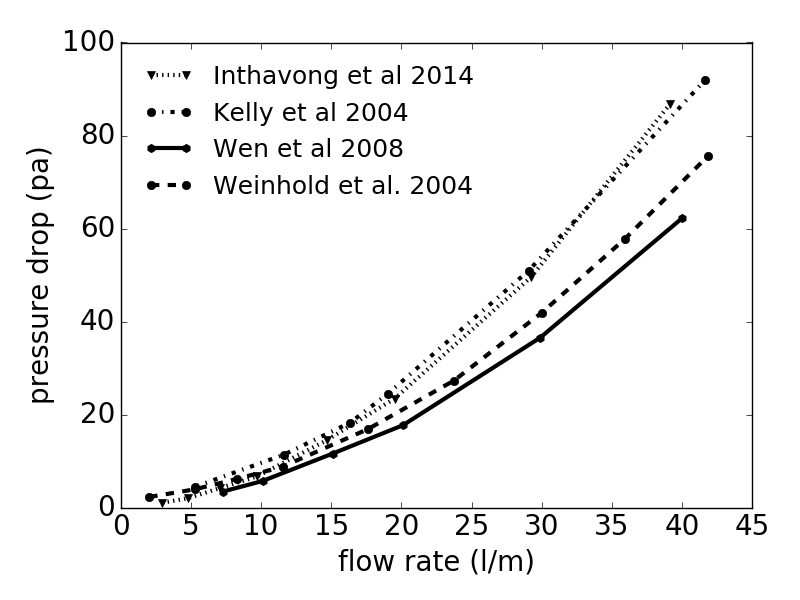
\includegraphics[width=0.8\textwidth]{pressureDrop.png}
  \caption{Pressure drop across the nasal cavity as a function of flow rate} \label{fig:pvf}
\centering
\end{figure}

 \subsubsection{Wall shear stress and velocity}

Velocity distributions in the nasal cavity play a significant role in olfaction \cite{Ishikawa2009} and Particle filtration \cite{Inthavong2006, Wang2009a} as well as general understanding of nasal function \cite{Keyhani1995, Zhu2011, Lintermann2013}. 
These can be examined by cross sectional zone by zone analysis \cite{Keyhani1995, Zhu2011}, which has been suggested to be useful for the measurement of the efficacy of olfaction \cite{Zhu2011}, or by longitudinal sections \cite{Lintermann2013,Taylor2010}. 

It has been suggested that shear stress at the wall of the nasal cavity could impact on the complex multifarious histiological mechanisms contained in the nasal epithelium \cite{Elad2006}.
Distributions are analysed longitudinally \cite{Wen2008} or around the cross sectional parameter of the relevant section of the nasal cavity \cite{Burgos2014}. 

These measurements (Wall shear and velocity) have been shown to be significant for predicting heat and mass transfer characteristics \cite{Taylor2010}, and as such their longitudinal and parametric distributions are significant for understanding the distribution of such mechanisms. 

\begin{figure}
  \centering
  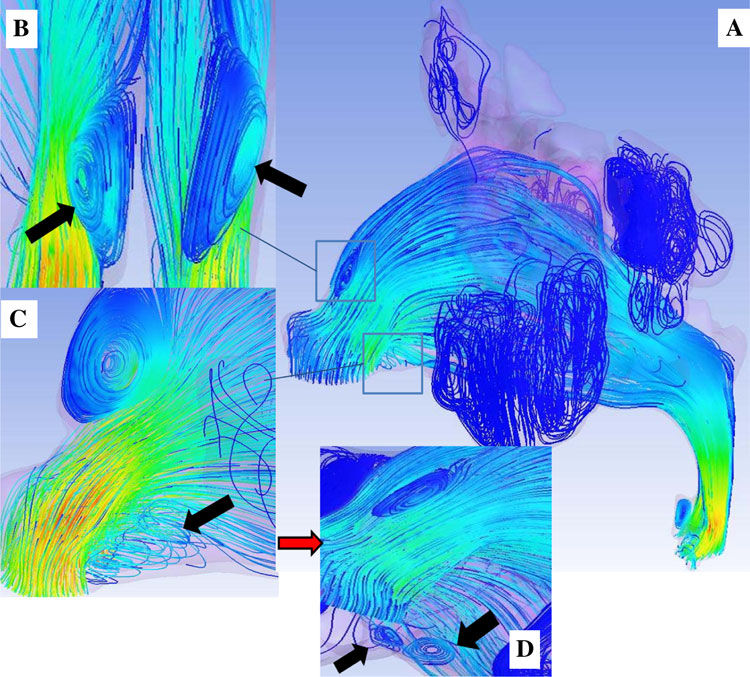
\includegraphics[width=0.6\textwidth]{chinstreams.png}
  \caption{Inspiratory airflow streamlines in the nasal cavity with sinuses coloured by velocity from Tan et al. \cite{Tan2012}} \label{fig:chinstreams}
\centering
\end{figure}

\begin{figure}
  \centering
  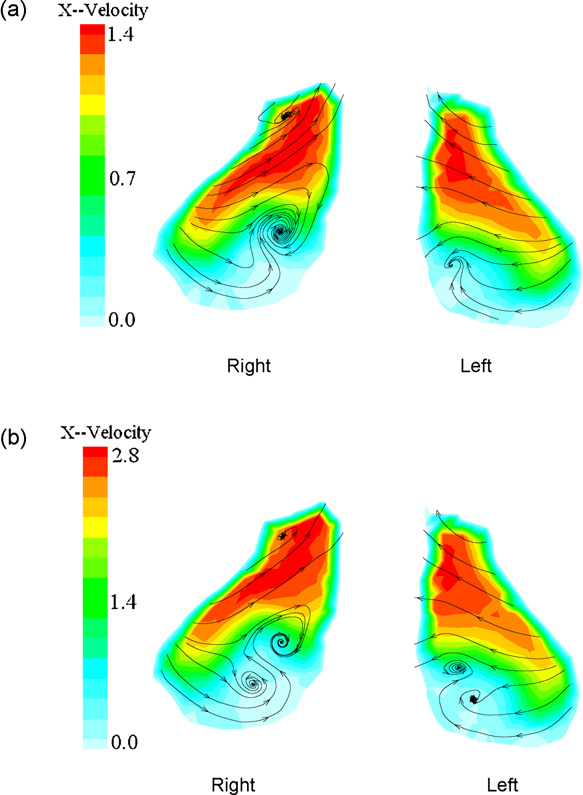
\includegraphics[width=0.4\textwidth]{wencont.png}
  \caption{Velocity contours at the nasal valve for steady state inspiratory flow rates of a) 7.5 lpm and b) 15 lpm from Wen et al. \cite{Wen2008}} \label{fig:wencont}
\centering
\end{figure}

One common visualisation method is the use of streamlines (shown in Figure \ref{fig:chinstreams}). Streamlines, often coloured by velocity \cite{Wen2008, Zhu2011, Garcia2007}, are useful for showing flow distribution as well as significant recirculation zones \cite{Lintermann2013, Xi2014}. Another commonly used method, shown in Figure \ref{fig:wencont} is coronal cross sectional contours coloured by velocity. These contours may or not include streamlines to help highlight the presence of vortices in the flow \cite{Wen2008}. Another method, presented in Lintermann et al. \cite{Lintermann2013} uses a vortex detection algorithm to trace the vortices present in the flow structure. In Lintermann et al. \cite{Lintermann2013}, these are then coloured by variables related to turbulence and vorticity in order to provide a deeper insight in to the vortex structure and behaviour.

\subsubsection{Heat and vapour transfer}

The conditioning of inhaled air - by both humidification and heating - in preparation for interaction with the sensitive tissues of the respiratory system is one of the primary functions of the nasal cavity \cite{Elad2008}.
Under standard atmospheric conditions, the air reaches an average temperature around 34\degree C and humidity of 32 $mg H_2 O/l$ by its entrance to the pharynx \cite{Keck2000}.
Interethnic variations in Nasal airconditioning effectiveness have been observed and suggested to be linked to climate related evolutionary variations \cite{Noback2011, Yokley2009}.
Reductions in airconditioning functionality in older patients have been observed experimentally \cite{Lindemann2008}.
The average temperature of the respiratory epithelium during resting nose breathing has been found to be 32.6$^{\circ} C$ \cite{Lindemann2002}.

Earlier investigations into the heat and vapour transport characteristics of the nasal cavity used a straight pipe model as a simplification of the nasal cavity geometry \cite{Ingelstedt1961}. The first experiments involving real nasal cavity geometries were carried out in the 80s, using cast models taken from cadavers \cite{Nuckols1983}.

In vivo experiments into temperature variation across the nasal cavity have been done using various temperature measuring devices; modern experiments have tended towards using thermocouples because they are small and respond quickly \cite{Elad2008}. For measuring humidity in vitro, modern researchers have tended towards the use of capacitative humidity sensors \cite{Keck2000}. Detailed profiles of temperature and humidity throughout the nasal cavity have been presented by several past researchers \cite{Keck2000}. 

CFD has been used to simulate heat and vapour transfer in the nasal cavities with good accordance with experimental results \cite{Lindemann2004}. Early simulations investigating heat and vapour transfer used a steady state assumption for inflow conditions \cite{Naftali1998}. Later, the effect of the nasal cycle on temperature distributions was investigated, showing significant variations in the nasal temperature distributions throughout the nasal cycle \cite{Elad2006}. For these simulations, the respiratory epithelium, which coats the majority of the nasal cavity, was assumed to be at 100\% relative humidity, with the exception of the interior of the nostrils, for which there was zero water flux \cite{Elad2006}.

Coronal cross section temperature contours have been used to visualise the distribution of temperature throughout the nasal cavity; this provides a clear method for visualising the distribution of temperature throughout the cross section \cite{Naftali2005}. Sagittal heat flux contours have also been used to similar effect \cite{Sullivan2013}. Heat flux, temperature, water flux and humidity have all been mapped as functions of position across the sagittal axis in the nasal cavity \cite{Garcia2007, Sullivan2013, Yu2014}. The nasal valve has been noted from these observations to be a region of particular significance to heat and vapour transfer mechanisms \cite{Sullivan2013}. 

In vivo studies looking at older nasal cavities have shown them to exhibit a reduced humidifying and heating capacity \cite{Lindemann2008}. Further investigations through computational methods into these variations could lead to more insight into the mechanisms underlying these discrepanies.

\subsection{Demographic studies}
One common application of CFD and fluid dynamics in rhinology is to investigate the effects of interdemographic variations in nasal geometry on flow features. The previously investigated demographics include ethnicity \cite{Zhu2011}; disease \cite{Garcia2007}; and  age \cite{Xi2012}. Age can be subclassified into children \cite{Xi2012} and the elderly \cite{Lindemann2008}. Both child and older nasal cavities have been investigated through in vitro \cite{Weinhold2004} and in vivo \cite{Kalmovich2005, Edelstein1996, WhanKim2007, Lindemann2008} experimental techniques. Child models have also been investigated computationally \cite{Xi2012}. The variations that have been observed in children's nasal airway functionality has been suggested to be linked to particle filtration ability \cite{Xi2012}. It seems plausible that this effect could be significant also in the case of elderly models. It is to date, however, unknown as in depth computational studies investigating flow field variations in older models are yet be undertaken.


\section{Summary}

Throughout this section, we have seen that the nasal cavity is an important organ for airconditioning as well as olfaction. We have seen that there are an assortment of ailments related to this organ which effect older patients in particular. It has been seen that there are clearly established trends between nasal cavit volume and age. We have examined the various methods available for examining the functionality of the nasal cavity. We have also looked at the use of fluid dynamics for classifying and understanding the functionality and pathology of the nasal cavity.

Although various experimental techniques have been used historically in rhinology, none of them provide the same cost effectiveness and level of detail which can be obtained through computational analysis of 3D models obtained from medical imaging. This method has been used extensively in recent years to examine various aspects of nasal cavity functionality, including interdemographic variations therein. These investigations have yielded multifarious insights into the various capacities of the organ. To date, to the best of my knowledge, the investigated demographics have not included older patients.

\section{Literature gap}

\begin{figure}
  \centering
  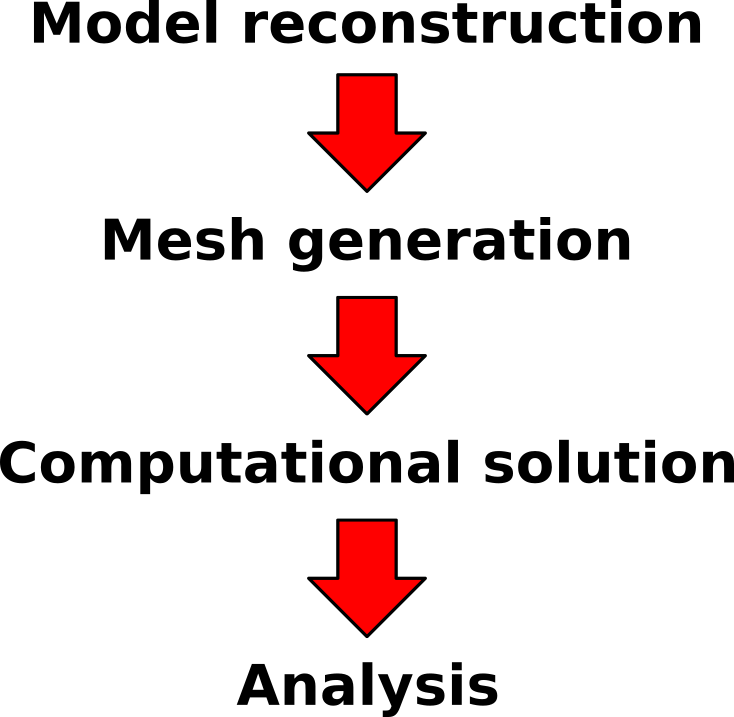
\includegraphics[width=0.6\textwidth]{probschem.png}
  \caption{Schematic overview of research}\label{fig:prbschm}
\centering
\end{figure}

On the basis of the literature review presented above, the following gaps in the current body of knowledge seem significant:

\begin{itemize}

  \item Detailed analysis of geometric discrepencies between older nasal cavities based on 3D scan models are yet to be carried out

  \item The correlations between geometric discrepencies in older nasal cavities and the airflow mechanisms induced in them through inspiration has yet to be analysed

  \item The effect of geometric discrepencies between older nasal cavities on heat and vapour transfer has yet to be assessed in detail

\end{itemize}
\section{Research questions and objectives}

In light of the information posed above, the following questions become pertinent:

\begin{itemize}

  \item How do variations in nasal cavity geometry in older Chinese Males influence the inhaled airflow mechanisms, contributing to respiratory ailments?

  \item How do the geometry variations impact on heat and vapour transfer within the cavity, contributing to respiratory ailments?

\end{itemize}

To address these issues, the following objectives are outlined:

\begin{itemize}

  \item Reconstruct a series of nasal cavity geometries from medical scans that represent a spread of geometric characteristics [such as volume and surface area] across the norm. The existing literature shows a clearly defined relationship between age and volume: these models will serve as a representative sample of the older population to be analysed computationally.

  \item Model airflow across the series of reconstructed nasal cavities using CFD with a steady state assumption; defining inlet conditions to approximate a resting rate of respiration. 

  \item Compare the simulation results between geometries. A variety of post processing methods are available to compare various aspects of fluid mechanic functionaility of nasal cavity models. The literature has shown clear discrepencies in the functionality of nasal cavities as a function of age; it is our intention through these measurements to examine in more detail the relationship between these variations and geometry.

  \item  Compare with results from the literature. 
\end{itemize}
 
\section{Research overview}

Medical image reconstruction technologies now allow researchers to reconstruct highly detailed, digital 3D representations of various anatomical structures from ct scans. When coupled with CFD simulations, this presents an unprecedented capacity for in depth analysis of physiological fluid flow mechanisms.

This study aims to use CFD analysis of CT scan data from the nasal cavities of a range of older Asian males to investigate the impact of geometric variations between older nasal cavities on the airflow structures and air-conditioning capacity of the nasal cavity. Air flow mechanisms, heat transfer rates and humidification efficacy are analysed in order to arrive at a more precise understanding of the role of nasal geometry in the presentation of respiratory ailments.

This study represents, to the best of our knowledge, the first in depth, mechanistic, computational study undertaken into the role of nasal geometry in common rhinological symptoms observed in older patients.






%\chapter{Literature review}
%
%
\section{Geriatric rhinology}
The common rhinological complaints of the elderly include dryness, runny noses, crusting and epistaxis\cite{Varga-Huettner2013}. Epidemiological studies have been carried out to examine the consistency of the manifestation of various symptoms throughout elderly patients with mixed results. 

The literature at present seems to be unanimous on the tendency of the nasal cavity's cross sectional area to increase with age. Several researchers have investigated this phenomena using acoustic rhinometry and shown good concordance in study outcomes\cite{Kalmovich2005, Edelstein1996,WhanKim2007,Lindemann2008}. Loftus et al. \cite{Loftus2016} compared the volumes of 22 nasal cavity models taken from CT scan data, and also found a clear tendency towards increased nasal cavity volume with ageing. Nasal air heating and humidification examined in vivo have been shown to be impaired by ageing\cite{Lindemann2008}. 

Increases in postnasal drip, nasal drainage, sneezing, coughing, olfactory dysfunction and gustatory rhinitis with age were observed in a clinical study of 131 patients\cite{Edelstein1996}. The results on the impact of aging on the quality of life have not been unanimous, a 2009 study found that in a sample of 80 people no significant relationship could be observed between age and nasal discomfort\cite{Lindemann2010}. The same study, however, concurred with previous results on the increase of volume and cross sectional area as a function of age. Changes within the nose appear to not be limited to the increased volume; Both functional and structural variations in the respiratory epithelium have been observed with age, contributing to slower clearing of mucous\cite{HO2001}. 

Functional variations in air conditioning capabilities have been shown in vivo\cite{Lindemann2008}, with statistically significant reductions in relative humidity and heat transfer observed in elder nasal cavities. The level to which this is attributable to change in histological function as opposed to variations in the fluid mechanisms as a result of the expansion of the cavity remains to be investigated.

 \section{Experimental Methods in Rhinology}
The anatomy of the nasal cavity was first classified in detail by Emil Zuckerlandl in the 19th century\cite{Stammberger1989}. Anatomically, his records were more or less up to the standard of what can be assessed from modern scanning techniques\cite{Stammberger1989}, however the investigation of airflow characteristics was still severely limited by technological capacity\cite{Eccles2000}. It was not until the turn of the 19th century that experimentation in to nasal airflow began in proper\cite{Eccles2000}. 

Some of the more common in vivo techniques used include rhinomanometry, which allows measurement of the pressure drop across the nasal cavity\cite{Hilberg1989} and acoustic rhinometry, which allows measurement of the cross sectional area of the nasal cavity as a function of depth\cite{Hilberg1989}. 

Ultimately, however, direct detailed measurements of flow mechanics within the human nasal cavity taken in vivo are not practically viable with current technology as a result of the complexity and small scale of the nasal geometry\cite{Doorly2008c}. Thus the preferred media for the testing in modern times has tended to be either physical or computational models reconstructed from CT scan data\cite{Doorly2008c}. The physical models that have been constructed from CT scan data are able to provide detailed geometric reproductions. These allow for much more detailed flow analysis when compared with older techniques such as rhinomanometry\cite{Ma2009}. Such experimental set ups are, however, costly to run in terms of time and resources, in particular when compared with the high level of detail that can be achieved from a well done CFD simulation\cite{Ma2009}.

\section{Computational Methods}
Computational fluid dynamics(CFD) is a discipline which is concerned with the computational approximation of solutions to the navier stokes equations for closed fluid systems\cite{Tu2008}. In many fields - inlcuding rhinology - CFD has facilitated economical and detailed investigations in to cases in which experimental investigation would otherwise be costly or impossible\cite{Keyhani1995}.

CFDs were the primary driving force behind the development of larger and faster computers until the 80's\cite{Wendt2009}. In more recent times, the continuing advancement of computational technologies has facilitated considerable growth in the scope and accuracy of CFDs for predicting the behaviour of increasingly complex systems\cite{Tu2008}. 

One of the areas of investigation that has been facilitated by these advances is that of nasal airflow. Initially, simplified nasal cavity geometry models were used to create computational meshes and solve numerically for the fluid flow characteristics under steady state state conditions\cite{Keyhani1995, Hahn1993}. Later 3D models extracted from CT scans were used to achieve more accurate results\cite{Martonen2002}. In addition to this, various inlet and outlet conditions have been considered, including the difference between unsteady state  (flowrate as a function of time throughout the nasal cycle)\cite{Shi2006} and steady state (constant velocity, time independent) assumption based models\cite{Wen2008}. This discrepancy has been a point of much contention, and it seems that the current position is that the correct choice depends on the application at hand\cite{Doorly2008c}. Certainly to date it seems that the vast bulk of the case studies comparing different geometries have used the steady state state assumption\cite{Xi2012, Zhu2011, Garcia2007}

Another issue which has been of some debate in the literature is the relevance of the inclusion of sinuses in the modelled flow domain. It has been reasonably commonplace to include the sinuses in studies that are examining the effects of sinus surgery\cite{Xiong2008a, Lindemann2005}. Also it has been shown that, while the impact on airflow is relatively minimal, the sinuses can be subject to significant levels of particle deposition for particles in the range of 1 nanometre in diameter, and particularly for low flow rates\cite{Ge2012}. The added requirements in time and computational complexity necessitated by the inclusion of the sinuses, however, seems to warrant their exclusion from models in situations where they are not specifically relevant\cite{Doorly2008c}


\subsection{Airflow structures}

\begin{figure}
  \centering
  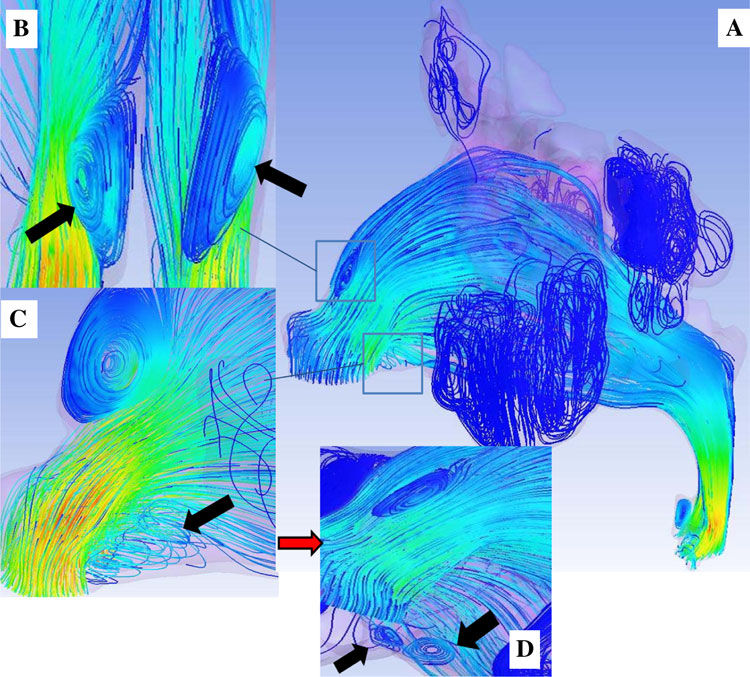
\includegraphics[width=0.5\textwidth]{chinstreams.png}
  \caption{Streamlines coloured by velocity from \cite{Tan2012}} \label{fig:chinstreams}
\centering
\end{figure}

\begin{figure}
  \centering
  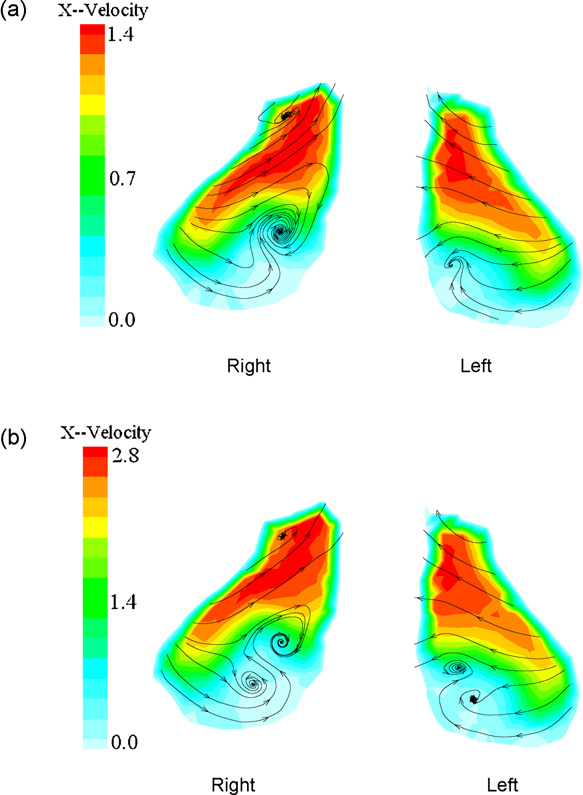
\includegraphics[width=0.5\textwidth]{wencont.png}
  \caption{Velocity contours at the nasal valve from \cite{Wen2008}} \label{fig:wencont}
\centering
\end{figure}
Airflow structures have been investigated and portrayed through a variety of both qualitative and quantitative methods. The earliest papers focused primarily on the pressure drop over the nostrils as measured with rhinomanometry\cite{Martin1981}. Modern technological innovation has facilitated the development of a range of techniques for both visualisation of airflows and the quantification of their various characteristics. In particular the range of data that can be obtained from numerical simulations is vast and detailed, and so the question of how to interpret it becomes particularly important.

One more commonly used visualisation method is the use of streamlines (shown in figure \ref{fig:chinstreams}). Streamlines, often coloured by velocity\cite{Wen2008, Zhu2011, Garcia2007}. These are useful for showing flow distribution as well as significant recirculation zones\cite{Lintermann2013, Xi2014}. Another commonly used method, shown in figure \ref{fig:wencont} is coronal cross sectional contours portraying velocity. These contours may or not include streamlines to help highlight the presence of vortices in the flow\cite{Wen2008}. Another method, presented in \cite{Lintermann2013} uses a $\Delta$ criterion to trace the vortices present in the flow structure. In \cite{Lintermann2013}, these are then coloured by variables related to turbulence and vorticity in order to provide a deeper insight in to the vortex structure and behaviour.

Quantitative methods for analysing and comparing air flow structures seem to be less standardised. Prior to the invention of modern imaging techniques, rhinologists relied on readings of cross sectional area and pressure from techniques such as rhinomanometry and acoustic rhinometry\cite{Doorly2008c}. The detailed flow information that can be extracted from CT scan models either experimentally or computationally opens up a much wider range of options in terms of quantitative analysis. Pressure is still often included as it is said to provide an insight in to the inspirational efficiency of the cavities\cite{Lintermann2013}. Pressure is often plotted as a function of flow rate in order to provide a point for validation by comparison with experimental set ups\cite{Wen2008, Inthavong2014}. In addition, it can be treated as a function of longitudinal position in order to gain an insight in to the relationship between the geometric variations and pressure drop\cite{Lintermann2013}. Another commonly measured variable is velocity distribution\cite{Keyhani1995, Zhu2011, Lintermann2013}. This can include cross sectional zone by zone analysis\cite{Keyhani1995, Zhu2011}, which has been suggested to be useful for the measurement of the efficacy of olfaction\cite{Zhu2011}, or by longitudinal sections\cite{Lintermann2013,Taylor2010} . Another commonly used quantitative measure is wall shear stress. Distributions are analysed longitudinally\cite{Wen2008} or around the cross sectional parameter of the relevant section of the nasal cavity\cite{Burgos2014}. These measurements have been shown to be significant for predicting heat and mass transfer characteristics\cite{Taylor2010}, and as such their longitudinal and parametric distributions are significant for understanding the distribution of such mechanisms.
 
\subsection{Demographic studies}
The previously investigated demographics include ethnicity\cite{Zhu2011}; disease\cite{Garcia2007}; and  age\cite{Xi2012}, which can then be subclassified into children\cite{Xi2012} and the elderly\cite{Lindemann2008}. Both of these have been investigated through both in vitro\cite{Weinhold2004} and in vivo\cite{Kalmovich2005, Edelstein1996, WhanKim2007, Lindemann2008} techniques. Child models have also been investigated computationally\cite{Xi2012}. The variations that have been observed in children's nasal airway functionality has been suggested to be linked to particle filtration ability \cite{Xi2012}. It seems plausible that this effect could be significant also in the case of elderly models. Cross sectional areas have been graphed as a function of radial position to compare the geometries of different models in many studies\cite{Xi2012, Zhu2011, Lindemann2008, Garcia2007}. Surface area has also been suggested to be significant metric in predicting flow behaviour (as surface area to volume ratios are expected to impact on the flow behaviour\cite{Xi2012, Garcia2007}). Resistance across the nasal cavity, measured as pressure drop, is also often used as a predictor of flow behaviour within the nasal cavity\cite{Edelstein1996, Lindemann2008, WhanKim2007}. As previously stated, streamlines are a commonly used method for visualising flow structures in nasal cavity models. They have as such been used in several instances to compare interdemographic variations in flow structure\cite{Xi2012, Garcia2007, Zhu2011}. Flow flux by saggital section across the turbinal region has also been used to identify variations in nasal functionality\cite{Zhu2011}. 


\subsection{Heat and vapour transfer}

Earlier investigations in to the heat and vapour transport characteristics of the nasal cavity used a straight pipe model as a simplification of the nasal cavity geometry\cite{Ingelstedt1961}. The first experiments involving real nasal cavity geometries were carried out in the 80s, using cast models taken from cadavers\cite{Nuckols1983}.

In vivo experiments into temperature variation across the nasal cavity have been done using various temperature measuring devices; modern experiments have tended towards using thermocouples because they are small and respond quickly\cite{Elad2008}. For measuring humidity in vitro, modern researchers have tended towards the use of capacitative humidity sensors\cite{Keck2000}. Detailed profiles of temperature and humidity throughout the nasal cavity have been presented by several past researchers\cite{Keck2000}.

CFD's have been used to simulate heat and vapour transfer in the nasal cavities with good accordance with experimental results\cite{Lindemann2004}. Early simulations investigating heat and vapour transfer used a steady state assumption for inflow conditions\cite{Naftali1998}. Later, the effect of the nasal cycle on temperature distributions was investigated, showing significant variations in the nasal temperature distributions throughout the nasal cycle\cite{Elad2006}.

Cross sectional temperature contours have been used to visualise the distribution of temperature throughout the nasal cavity; this provides a clear method visualising the distribution\cite{Naftali2005}. Saggital heat flux contours have also been used to similar effect\cite{Sullivan2013}. Heat flux, temperature, water flux and humidity have all been mapped as functions of position across the saggital axis in the nasal cavity\cite{Garcia2007, Sullivan2013, Yu2014}. The nasal valve has been noted from these observations to be a region of particular significance to heat and vapour transfer mechanisms\cite{Sullivan2013}. 




%\cite{Elad2008}
%
%in vitro studies - blood and mucous as transport agents for heat and moisture. Ingelstedt and Tolmalm, 1961, straight pipe simulation. Casting plastic Nuckols et al 1983, napthalene sublimation - Hanna and scherer, 1986. 
%
%In vivo studies - limited due to complexity of geometry, posterior Temperature 31-34 deg C, 90-95\%, Keck et al 2000 a, b. Variation of the nasal mucosa temperature, turbulence linked to higher heat flux values - Lindemann et al 2002. Temporal change in cavity flow - Eccles 2000; Hanif et al. 2000
%
%Computational - accurate 3d replica for predicting temperature distribution - Lindemann et al 2004, 2006, Pless et al 2004a, 
%
%Naftali et al. 2005, full 3d model for heat and vapour transfer in anatomical replica
%
%Wolf et al 2004 - psychometric charts used to calculate required heat and water to condition incoming air
%
%Naftali et al 2005 - varied inlet conditions show similar conditining capacity
%
%Kastl et al - impact of rhino-surgical interventions
%
%Influence of septal deviations - Pless et al. 2004b
%
%
%\cite{Garcia2007}
%
%Heat flux adjusted for evaporation as per (40)
%
%100\% RH at wall due to mucus
%
%vestibule zero water flux
%
%ambient air at 50\% RH, outflow at outlet
%
%mapped temperature across cavities, also relative humidity, water flux contours
%heat flux and water flux against length. Also as a function of height from nasal floor
%
%Tables of water flux per unit area
%
%flow partitioning
%
%pressure drop


\section{Literature gap}

To date, to the best of our knowledge, although some research has been carried out on the effects of aging on nasal airflow, CFDs have not been used to examine in depth the influence of age related variations in nasal cavity geometry on flow structure or heat and vapour transfer characteristics in older nasal caities. 

%\section{Particle filtration}
%
%



\chapter{Model reconstruction and meshing} \label{MRM}

\section{geometry}
\subsection{Introduction}

The reconstruction of nasal cavity model computer images - including discretisation for modeling with CFD - can be divided into 5 stages: image aquisition, data conversion, segmentation, refinement and meshing. Firstly medical imaging technologies are used to extract a series of pixelated slices, in which the various materials which make up the human body can be identified by variation in greyscale measurements. These slices are then interpolated to create a 3D structure of voxels (the 3D equivalent of a pixel).

The reconstruction of the nasal cavity geometries can be very time consuming and prone to human error. The improvement on and automation of the reconstruction process are areas of active research. This chapter presents an overview of the methods in current use for the various phases (mentioned above) by which a nasal cavity geometry is prepared for CFD analysis.

\subsection{Non-invasive Medical Imaging}

There are various forms of medical imaging that can be used for the identification of the nasal cavity geometry. Here a brief overview of Computed Tomography (CT), the form of medical imaging used for the nasal cavity geometries presented in this thesis.

CT scans use a series of x-rays taken at regular intervals within the required region. x-ray scans use photons sent in beams through the region of interest. These photons interact differently with the material that they encounter depending on its density. Electronic detectors feed the photon pattern emitted from the body in question to a computer, which uses this information to create images. These images are made up of pixels which are each assigned a grey scale value based on their x-ray attenuation coefficient. In medical imaging the Hounsfield scale is used, whereas in image processing the greyscale is numbered from black to white between 0 to 255. Figure \ref{fig:greyscale} shows an  

\begin{figure}
  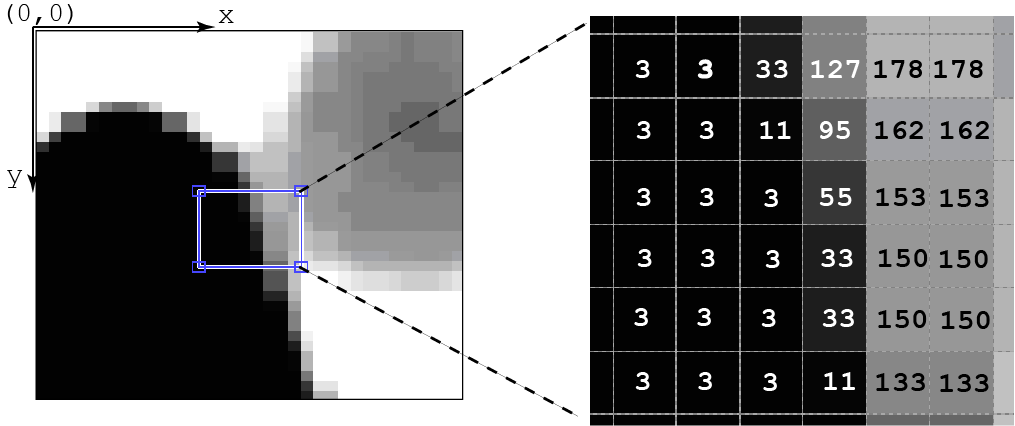
\includegraphics[width=1\textwidth]{grayscale.png}
\caption{example of how greyscale values are assigned to pixels in a ct image} \label{fig:greyscale}
\centering
\end{figure}
 
\subsection{Image Segmentation} 

On ce the CT scan has been outputted as a series of voxels, the anatomical geometries relevant to the project at hand can be extracted. To achieve this goal, the voxels that make up the relevant chapter of the data need to be identified somehow. This can be done manually - by going through the many slices that make up the ct scan and identifying the relevant areas - however this process is extremely time consuming.
\ subsection{Segmentation Methods}

Numerous algorithms have been developed for the purpose of automating the process; all of which have certain advantages and disadvantages. For the most part these algorithms can be subsumed in to three categories, presented below (in order of increasing complexity):

\begin{itemize}

  \item \textbf{Thresholding:} regions are identified and separated according their  greyscale value. This is the simplest algorithm for defining regions.

  \item \textbf{Edge detection:} either local maxima of the first derivite of intensity or zero values of the second derivative are used to identify region edges. Edge detection tends to reduce the noise when compared with thresholding

  \item	\textbf{Region based:} regions are grown from the inside out. This produces more coherent regions, but is unable to detect regions that are segregated.

\end{itemize}

These methods and many more exist and are in active development. In addition, many of them are available for free online. The implementation of such algorithms and applying from first principles, however is quite a complex procedure. Fortunately many of these algorithms have already been implemented in software packages - of which commercial and open source variations are available - which are specifically compiled for working with medical imaging outputs. 

\subsection{Preparation of Model for Meshing}

Once the region in question has been extracted from the medical imaging output, it can be saved as some CAD format. There are certain criteria that need to be fulfilled by a CAD model before it can be read by 3d meshing software and used to create a mesh. It is often the case that when the data is exported from the medical imaging software is 'dirty'; that there are contradictory or arbitrary elements in the geometry. These elements need to be removed through the use of CAD software before the geometry is suitable for the creation of a useable 'clean' 3d mesh. Note that the geometry needs to contain also topological information in order to create a watertight mesh. The details of the process by which the geometry is prepared for meshing are described in Figure \ref{fig:segchart}.


\begin{figure}
  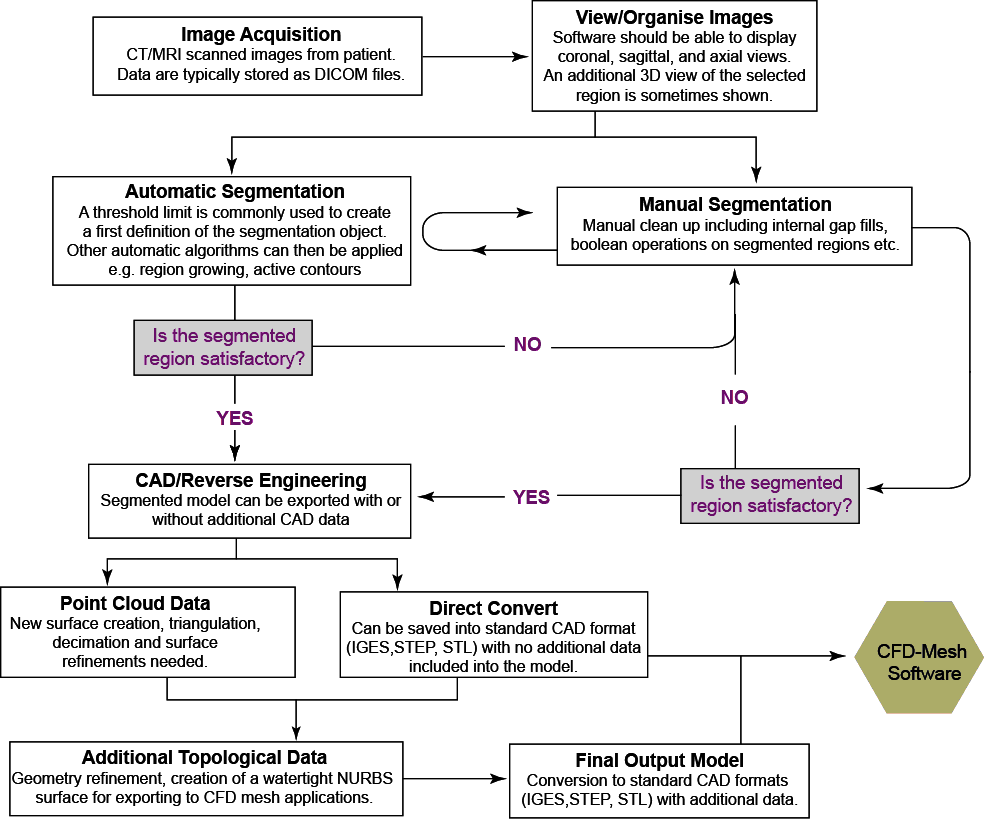
\includegraphics[width=1\textwidth]{flowchart.png}
\caption{Flow chart showing the process by which an anatomical geometry is prepared - with the help of medical imaging - for modeling with CFDs} \label{fig:segchart}
\centering
\end{figure}

\subsection{Summary} 

Anatomical geometry reconstruction - including that of respiratory systems - begins with medical imaging of the area in question. The geometry is then extracted from the medical imaging data using one (or several) of the available extraction algorithms outlined above. After extraction, cleaning of the geometry with CAD software is generally necessary. It is necessary to ensure that the geometry is water-tight before it can be meshed. This chapter has given an overview of some of the more pertinent methods in current use for the reconstruction of anatomical geometries from medical imaging data. Figure \ref{fig:cavzamp} shows an example of the construction process.

\begin{figure}[t!]

  \begin{subfigure}[t]{0.5\textwidth} 
    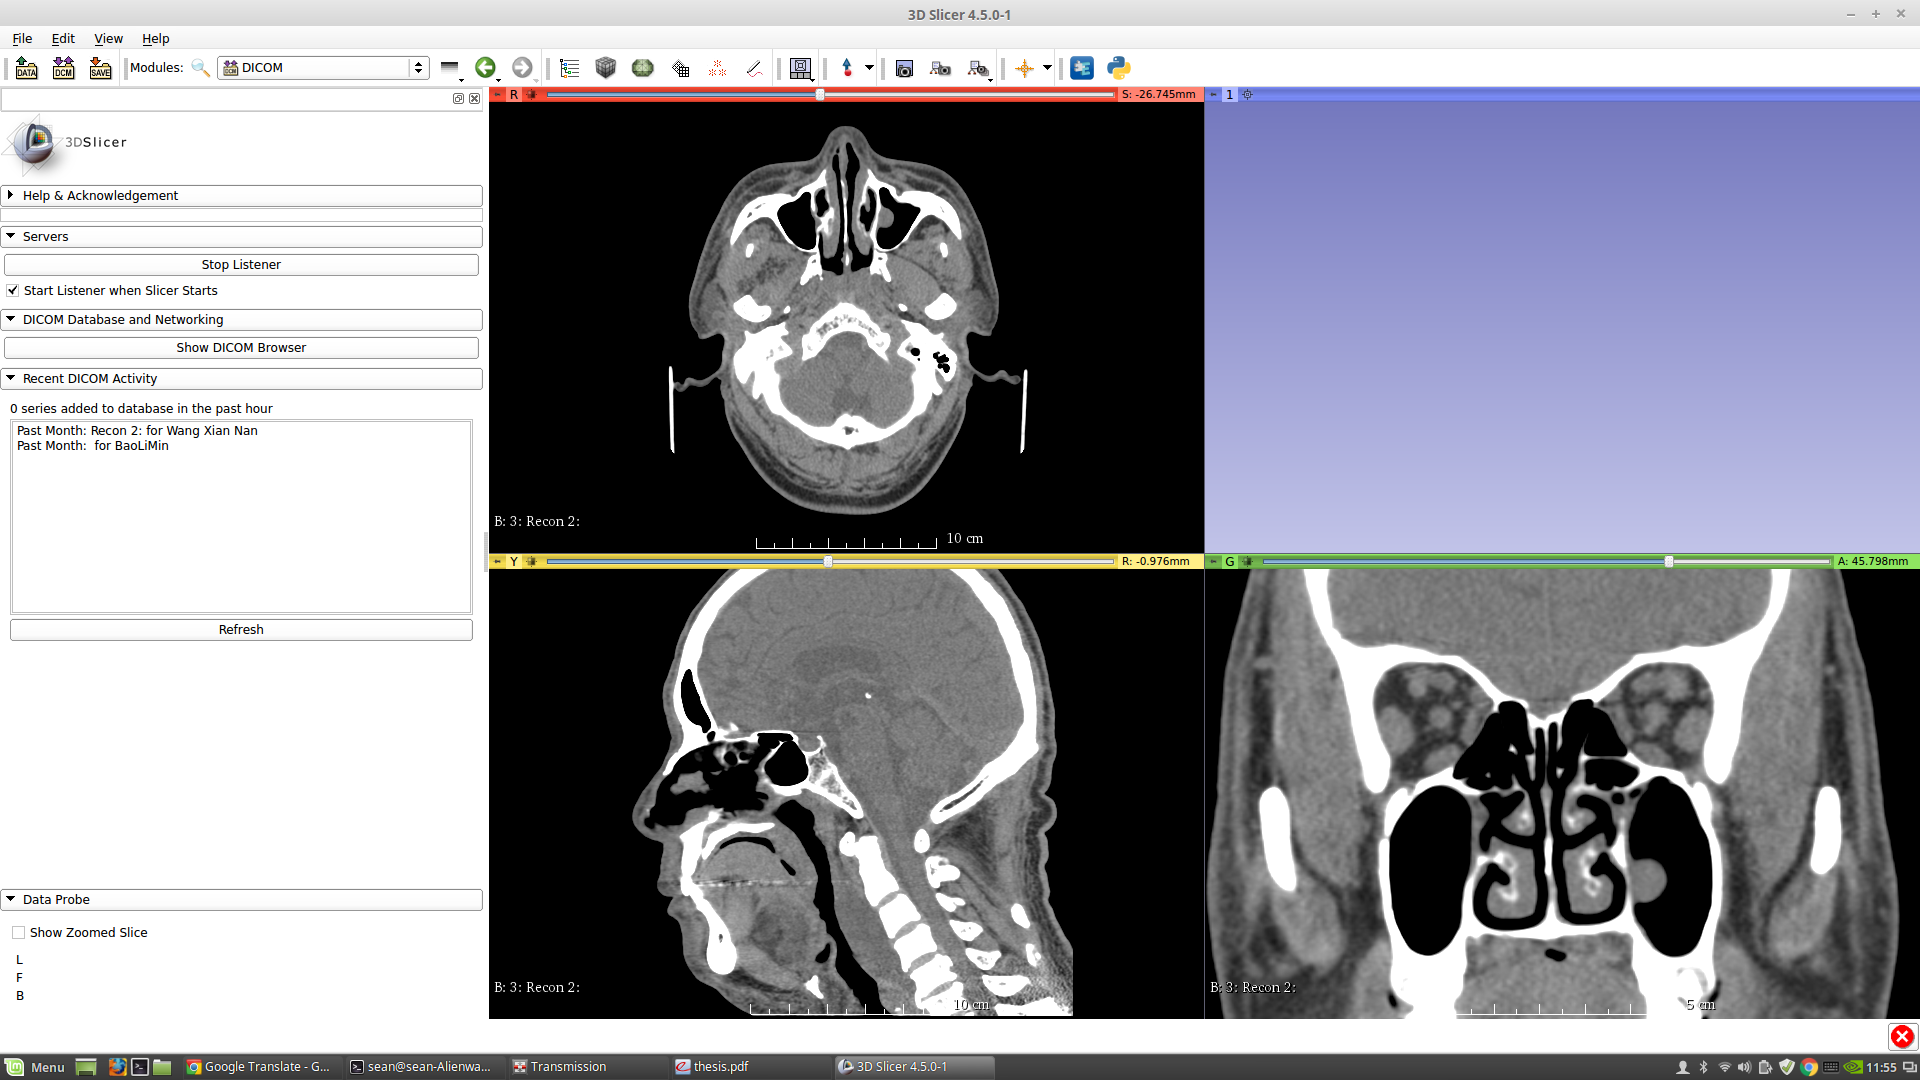
\includegraphics[width=\textwidth]{slicer}
    \caption{An example of the extraction of a 3D model from CT scan data, using, in this case, an open source software package, slicer}
    \label{fig:slicer}
  \end{subfigure}%
  ~ %
  \begin{subfigure}[t]{0.5\textwidth} 
    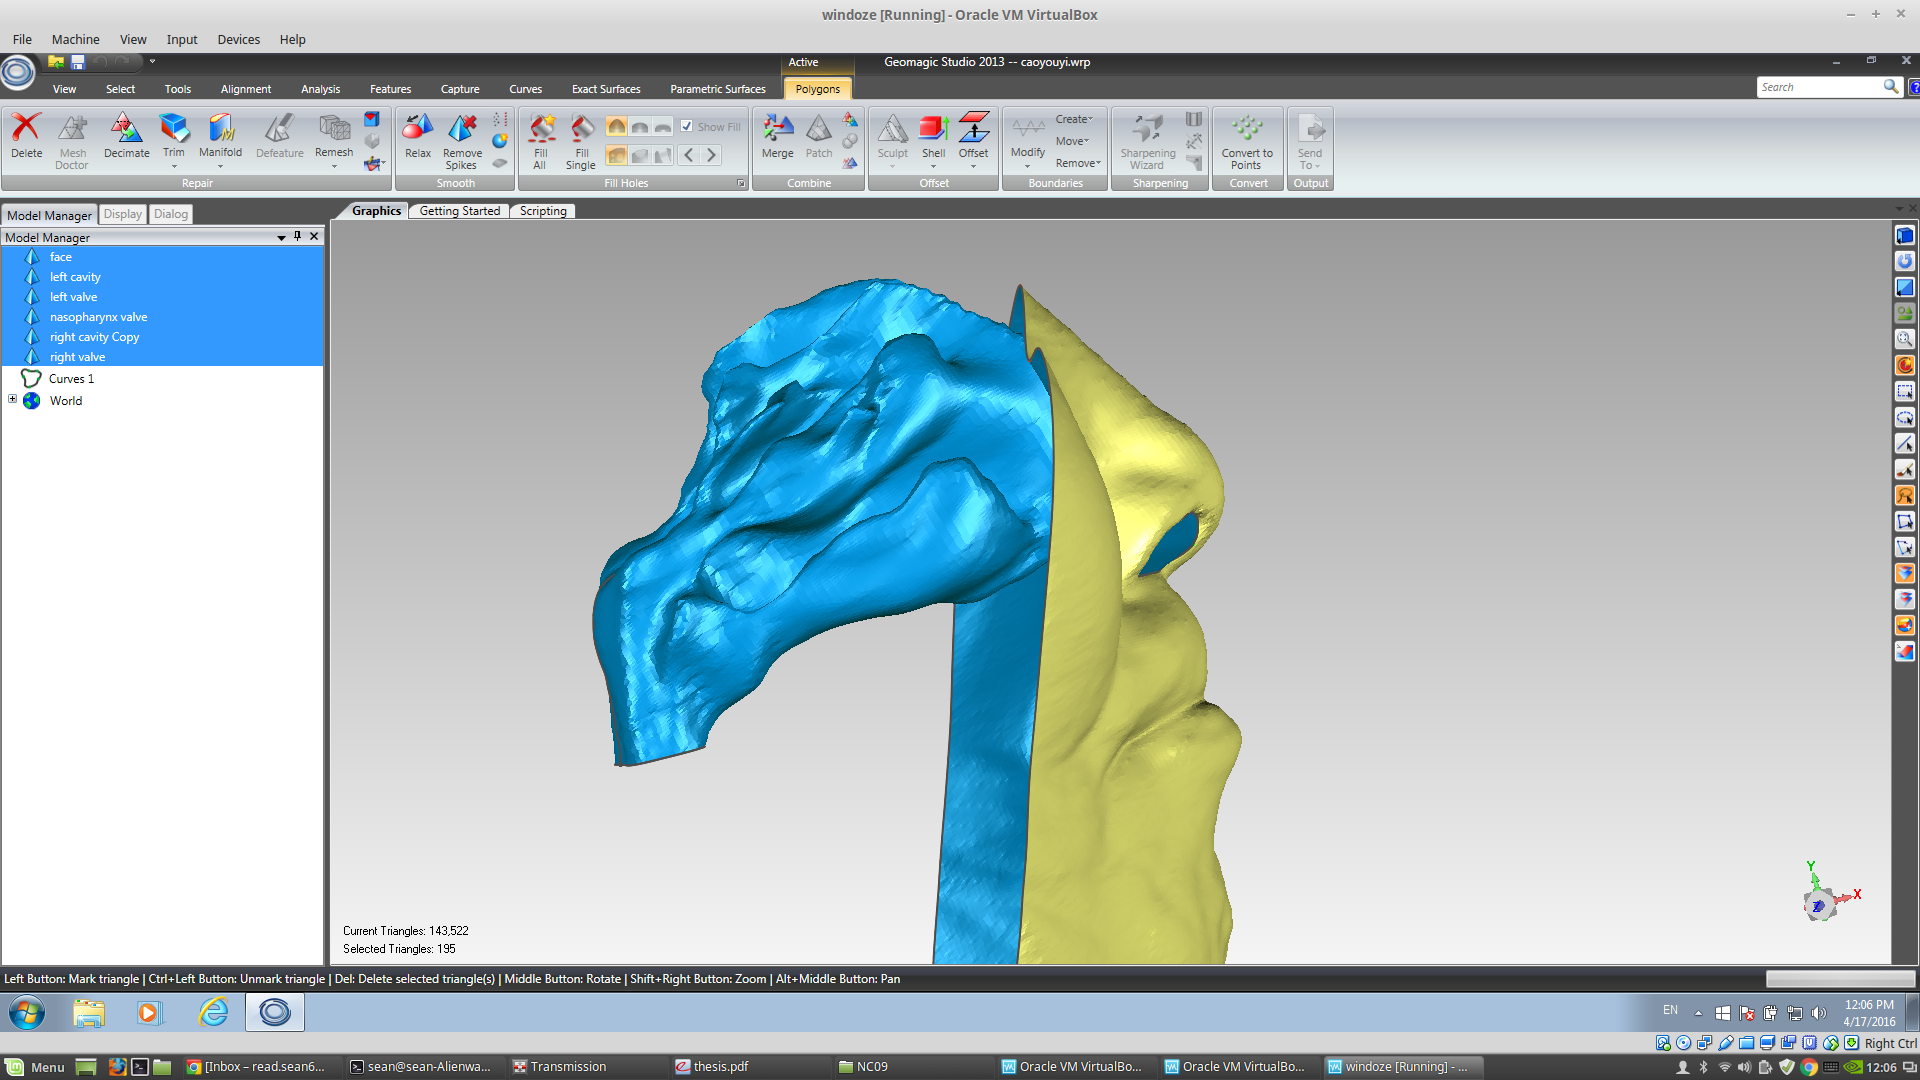
\includegraphics[width=\textwidth]{geomagic}
    \caption{the refined geometry extracted from the CT slices seen in figure \ref{fig:cavzamp} (\subref{fig:slicer})}
    \label{fig:geomag}
  \end{subfigure}

  \caption{Example of nasal cavity geometry generation}
  \label{fig:cavzamp}
\end{figure}
 
\section{Meshing}
\subsection{Introduction}

The navier stokes equations, upon which Computational Fluid Dynamics is based (see chapter \ref{cfd}), is unsolvable (in most instances), except by approximation. A given geometry is approximated, or discretised, as a series of points. The process by which these points are defined and related to one another is known as meshing; this in itself is a complex discipline under active research. In this chapter current methods are reviewed, and guidelines are given for developing quality meshes.

\subsection{Mesh Types} \label{mtypes}

There are many types of mesh structure that can be employed; all of them have their own advantages and disadvantages. 

\begin{itemize}
  \item{Structured meshes} 
    by definition, are divided into segments of uniform size and shape. It is characterised by cells posessing either four nodal corner points in two dimensions, or eight three. The points are mutually orthogonal and cartesionally defined. Being defined in this relatively simple way facilitates a higher level of computational efficiency. It is, however, limited in the level of structural complexity that it can accomodate.

  \item{Unstructured Meshes}
    The geometries encountered in the respiratory system are generally too complex to be effectively discretised in a structured manner; in cases such as these unstructured meshes can be used to acommodate the complexities of the given geometry. Unstructured meshes - usually constructed from triangles or tetrahedra - do not fit a regular pattern, and they do not have coordinate lines corresponding to curvilinear directions. Because of this, the solving of compuations over unstructured domains is generally more computationally intensive, however with modern advances in computers this has become less significant an issue in many cases.

  \item{Hybrid meshes}
    One disadvantage to the use of unstructured meshes is that they tent to show less accuracy near the wall. One commonly applied solution is the use of hexahedral elements near the wall, with the rest of the volume filled with unstructured - usually tetrahedral - elements. This method tends to improve the accuracy of near wall computations. One draw back of this method is that the prism layers can break down in the vicinity of excessively contoured walls. In this study this is the mesh type that is employed.

\end{itemize}

\begin{figure}

  \caption{Examples of the mesh types described in section \ref{mtypes}} \label{fig:struct}
\end{figure}

\subsection{Meshing algorithms}
There are various meshing algorithms available, each with their own strengths and weaknesses. For the purpose of this study, an octree algorith was selected. Octree algorithms work by repeatedly dividing The volume in to smaller sections, until the given criteria, for example mesh size, is fulfilled. This method is generally considered to be a relatively simple but robust approach to mesh generation. One drawback, however is that it can cause irregular element distributions near the boundary.

\subsection{Quality}

The quality of a generated mesh is dependant on its warp angle, skewness and aspect ratio. For a quadrilateral cell, as shown in figure \ref{fig:mqual}, the aspect ratio of the cell is defined as $AR = \frac{\Delta y} {\Delta x}$. Within the interior region, the $AR$ should be maintained within the range $0.2 < AR < 5$. This can be somewhat relaxed, however, in the vicinity of the wall.

Mesh skewness is defined as the extent to which it deviates in shape from the ideal. This is a squate for quadrilateral cells, or an equilateral triangle for triangle or tetrahedral cells. It is simple quantified for tiangles and tetrahedrals as $\frac{\theta ideal - \theta actual} {\theta ideal}$ (see figure \ref{fig:mqual} for theta).

Many grid generation packages contain specific algorithms and/or functions for improving mesh quality. The gradient of mesh size variation should not exceed 1.2, as higher variations can cause problems in convergance.

\begin{figure}
  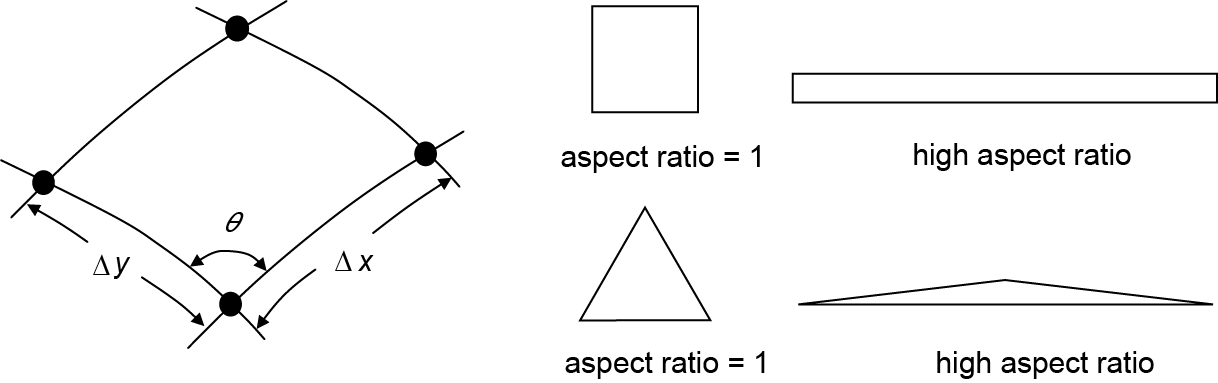
\includegraphics[width=1\textwidth]{mqual}
  \caption{Example of mesh cell with spacing $\Delta x$ , $\Delta y$ and angle $ \theta $ between the grid lines along with high $AR$ triangular and quadrilateral elements } \label{fig:mqual}
\end{figure}

\subsection{Mesh Independence}

A significant source of error in the solution of CFD problems is derived from the discretisation process; when a system is separated into a number of finite elements, for the purpose of Numerical solution, the solution that is obtained from its solution is an approximation. It is necessary, then, to ascertain the required resolution, or mesh size, required to calculate a result that approximates the exact solution to a satisfactory degree of accuracy. This is done by means of a mesh independence test. This entails the monitoring of one - or several - fluid flow parameters of interest to the study over a series of mesh sizes. Independence is said to have been achieved when the effect of mesh size on the selected flow variable(s) has become insignificant. Figure \ref{fig:mind} shows the results from the mesh independence test conducted for two of the five models presented in this thesis.

\begin{figure}

  \caption{mesh independence} \label{fig:mind}

\end{figure}
\subsection{Meshing of the Nasal Cavity}

Here we overview the meshing process applied to the nasal cavity models presented in this thesis.

The system is divided in to three parts. The first of these surounds the facial geometry directly adjacent to the nostrils; this is to allow the developement of a more realistic inlet profile. The second is the nasal cavity itself. The third section is an pipe-like extension from the exit of the nasopharynx; this allows for the developement of a more realistic outlet profile, in a similar manner to the section around the inlet. This system can be seen in figure \ref{fig:cavme} (\subref{fig:mesh1}).

The three stages of mesh refinement can be seen in figure \ref{fig:cavme} (\subref{fig:mesh2}); The mesh resolution is much coarser in the external domain, refined closer to the inlet and then is most fine in the cavity itself, the area of interest. Note the use of hybrid mesh, with internal tetrahedral elements and close to wall prism layers, shown clearly in Figure \ref{fig:cavme} (\subref{fig:mesh4}).

\begin{figure}
  \begin{subfigure}[t]{0.5\textwidth}
    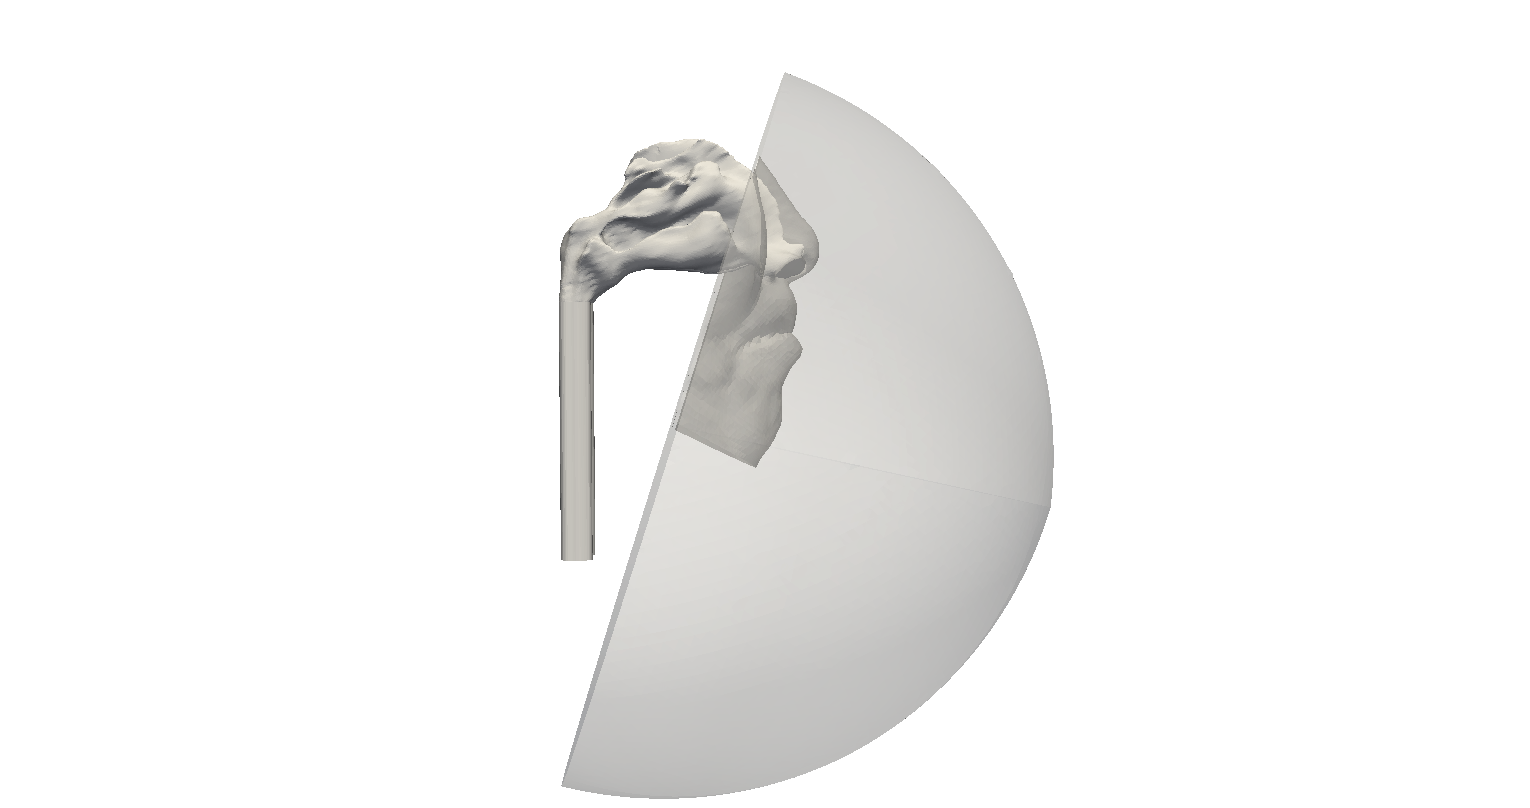
\includegraphics[width=\textwidth]{mesh2}
    \caption{whole system with face, extension from outlet and external zone}
    \label{fig:mesh1}
  \end{subfigure}%
  ~%
  \begin{subfigure}[t]{0.5\textwidth}
    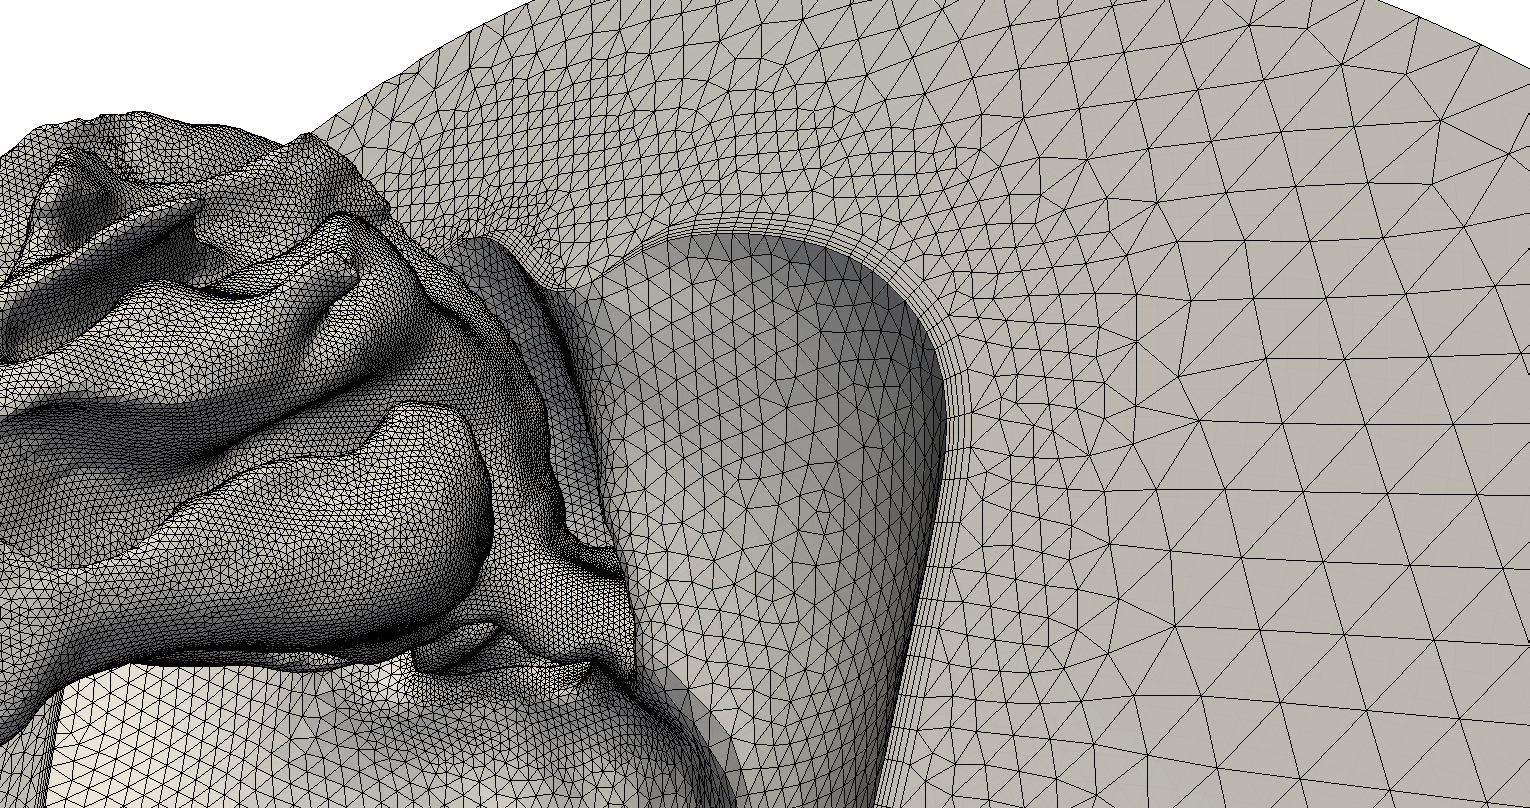
\includegraphics[width=\textwidth]{mesh1}
    \caption{intersection of three mesh resolutions}
    \label{fig:mesh2}
  \end{subfigure}

  \begin{subfigure}[t]{0.5\textwidth}
    
\includegraphics[width=\textwidth]{mesh3}
    \caption{cross section of cavity mesh}
    \label{fig:mesh3}
  \end{subfigure}%
  ~%
  \begin{subfigure}[t]{0.5\textwidth}
    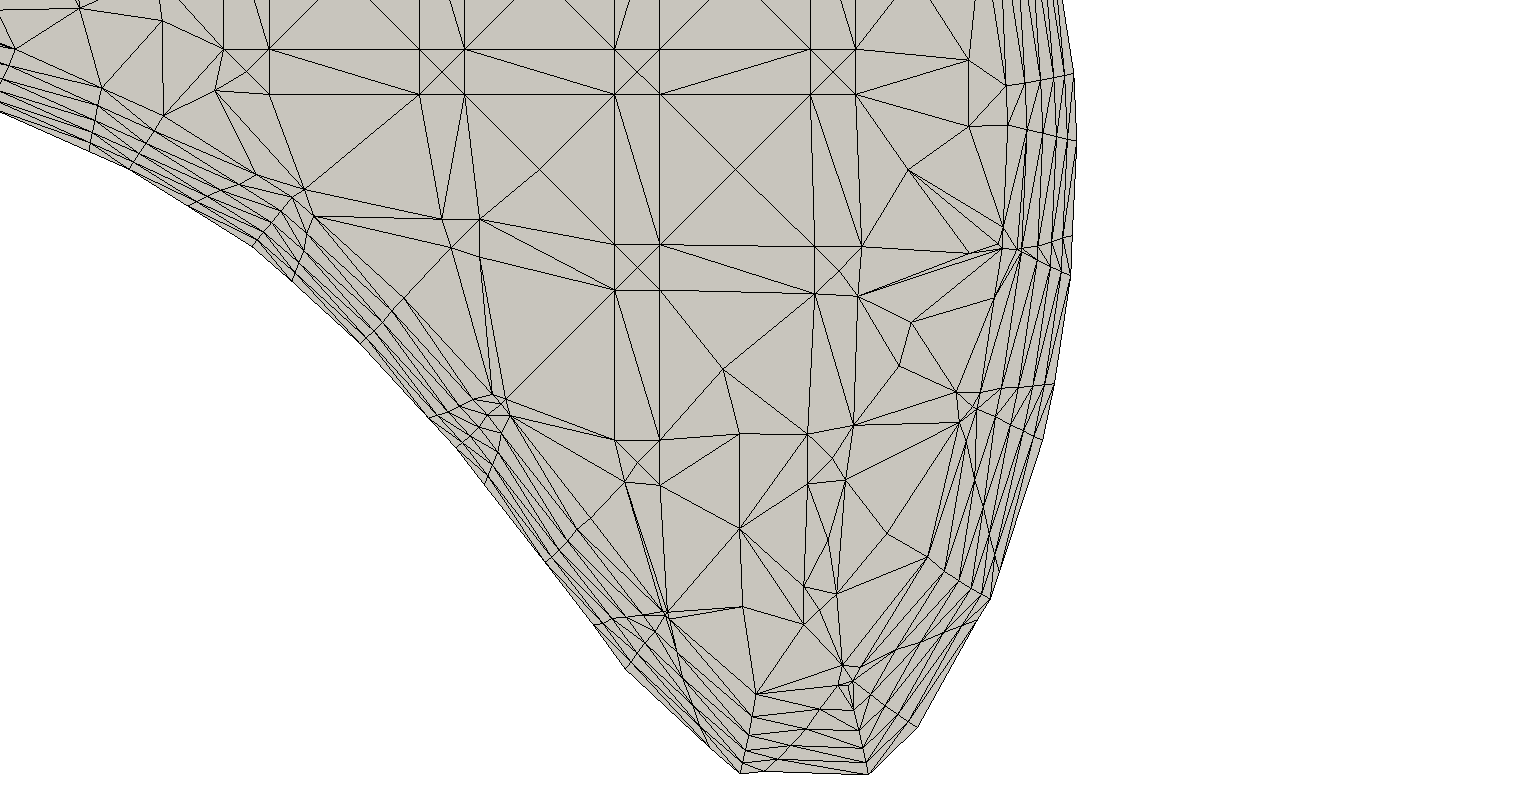
\includegraphics[width=\textwidth]{mesh4}
    \caption{prism layer of cavity mesh}
    \label{fig:mesh4}
  \end{subfigure}
  \caption{mesh of NC06} \label{fig:cavme}
\end{figure}


\chapter{CFD fundamentals} \label{cfd}

\section{Fluid Dynamics}
The aim of CFD is to numerically solve the physical conservation laws of newtonian physics:

\begin{itemize}
  \item Conservation of mass

  \item The conservation of momentum (Newton’s second law, the rate of change of momentum equals the sum of forces acting on the fluid);

  \item The conservation of energy (first law of thermodynamics, the rate of change of energy equals the sum of rate of heat addition to and the rate of work done on the fluid).
 
\end{itemize}

    \subsection{Mass conservation}

    The principle of conservation of mass is that, in a closed system, the mass remains constant. This means that fluid will move through a set region in such a way that the mass is conserved. For an incompressible flow, this means that the outflows and the inflows will be equal. This can be written as
    \begin{equation} \label{eq:1}
      0 = \sum_{in} \dot{m} - \sum_{out} \dot{m}
    \end{equation} 

    Where $\dot{m}$ = mass flow rate.
    
    The mass flow rate can be written as $ \rho u A $,  for $\rho$ = density, $u$ = velocity and A is the scross sectional area of the flow. For flow in the x direction, $ A = \Delta z \Delta x $. For a two dimensional flow, $ \Delta z = 1 $, giving:

    \begin{equation} \label{eq:2}
      \dot{m}_{in} = \rho u \Delta y
     \end{equation}

    Extending this to equation \ref{eq:1}, in the x direction, for an incompressible flow we get

    \begin{equation} \label{eq:3}
      0 = \rho u_{in} \Delta y_{in} - \rho u_{out} \Delta y_{out}
    \end{equation}

    This can easily be extrapolated to three dimensions.


Extending this further, in the x direction for the same two dimensional element we can say that

\begin{equation} \label{eq:22}
\dot{m}_{out} = [\rho u + \frac{\partial(\rho u)}{\partial x}\Delta x]\Delta y
\end{equation}

Applying this in the y direction and subsituting back into Equation \ref{eq:1}, for an incompressible flow we get
 
\begin{dmath} \label{eq:23}
0 = [\rho u + \frac{\partial(\rho u)}{\partial x}\Delta x]\Delta y - \rho u \Delta y 
+ [\rho v + \frac{\partial(\rho v)}{\partial y}\Delta y]\Delta x - \rho v \Delta x  
\end{dmath}

which then simplifies to

\begin{equation} \label{eq:24}
  0 = \frac{\partial(\rho u)}{\partial x} + \frac{\partial(\rho v)}{\partial y}
\end{equation}

which is the continuity equation, and can easily be extended into three dimensions as

\begin{equation} \label{eq:25}
  0 = \frac{\partial(\rho u)}{\partial x} + \frac{\partial(\rho v)}{\partial y} + \frac{\partial(\rho w)}{\partial z}
\end{equation}


    In the case of the nasal cavity, this can be conceptualised in relation to the nasal cavity geometry, where the air flow rate going into the nostrils must be equal to that leaving through the extension from the nasopharynx, as seen in figure \ref{fig:CompDom}.

\begin{figure}   
  \centering
  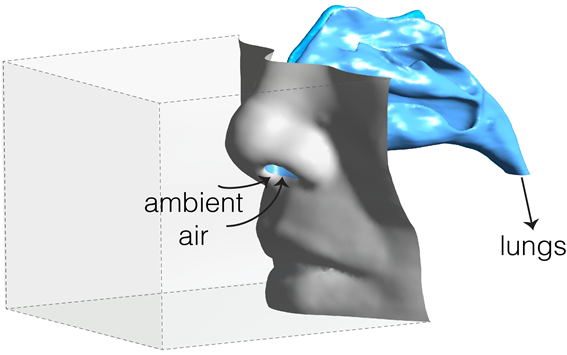
\includegraphics[width=0.5\textwidth]{CompDom}
  \caption{Fluid moving through the computational domain, the inflow of ambient air must be equal to the air entering the lungs}
  \label{fig:CompDom}
\end{figure}

    \subsection{Momentum conservation}

    Momentum conservation is based on the Newton's second law:

    \centerline{$\sum F = ma$}

    Here $m$ is the mass of the system, $a$ is its rate of acceleration, and  $\sum F$ is the sum of forces acting on the system. F can generally be divided into body and surface forces. Rewriting the mass as the product of volume and the density, and acceleration as the first derivative of velocity


    \begin{equation} \label{eq:4}
      \sum F_{body} + \sum F_{surface} = (\rho \Delta x \Delta y \Delta Z) \frac{DU}{Dt}
    \end{equation}

    Body forces generally include gravity, centrifugal, Coriolis and electromagnetic forces; these all act on the volume from a distance.

    Surface forces are those that act directly on the surface of a fluid element. These fluid forces include normal stress, in the x direction $\sigma_{xx}$, which is made up of pressure forces $p$ exerted on the body and normal viscous stress components $tau_{xx}$; and tangential stresses, $\tau_{xy}$ and $\tau_{xz}$.

    Summing these forces in the x direction, for a 2D fluid element we get
    

    \begin{dmath} \label{eq:5}
      \sum F_{surface, x} = [\sigma_{xx} \Delta y \Delta z - (\frac{\partial \sigma_{xx}}{\partial x} \Delta x) \Delta y \Delta z] 
      + [(\tau_{xy} + \frac{\partial \tau_{yx}}{\partial y} \Delta y) \Delta x \Delta z - \tau_{yx} \Delta x \Delta z]  
      = - \frac{\partial \sigma_{xx}}{\partial x} \Delta x \Delta y \Delta z + \frac{\partial \tau_{yx}}{\partial y} \Delta x \Delta y \Delta z
    \end{dmath}


    Assuming that the fluid is Newtonian and isotropic, $\sigma_{xx}$ can be related to pressure $p$ and viscous stresses $\tau_{xx}$ by

    \centerline{$\sigma_{xx} = -p + \tau_{xx}$}

    For a Newtonian fluid, stress-strain relations can be described as 

    \begin{equation} \label{eq:6}
      \tau_{xx} = 2 \mu \frac{\partial u}{\partial x} \quad \tau_{yx} = \mu \frac{\partial u}{\partial y}
    \end{equation}

    Where $\mu$ is the viscocity of the fluid. Combining equations \ref{eq:4} , \ref{eq:5} and \ref{eq:6} in the x direction, and cancelling out the volume term

    \begin{equation} \label{eq:7}
      \rho \frac{Du}{Dt} = - \frac{\partial p}{\partial x} + \mu (\frac{\partial^2 u}{\partial x^2} + \frac{\partial^2 u}{\partial y^2}) + \rho \sum F_{b}
    \end{equation}
    
    Here the acceleration term is the total derivative of u, defined as the combined local and advection inertial forces, which in two dimensions can be written as

    \begin{equation} \label{eq:8}
      \frac{Du}{Dt} = \frac{\partial u}{\partial t} + v \frac{\partial u}{\partial y} + u \frac{\partial u}{\partial x}
    \end{equation}

    combining equations \ref{eq:7} and \ref{eq:8} and dividing through by $\rho$

    \begin{equation} \label{eq:9}
      \underbrace{\frac{\partial u}{\partial t}}_{local\ acceleration} + v \underbrace{\frac{\partial u}{\partial y} + u \frac{\partial u}{\partial x}}_{convection} = - \underbrace{\frac{1}{\rho} \frac{\partial p}{\partial x}}_{pressure gradient} + \underbrace{\nu (\frac{\partial^2 u}{\partial x^2} + \frac{\partial^2 u}{\partial y^2})}_{diffusion} + \underbrace{\sum F_{b}}_{body force}
    \end{equation}

    Where $\nu$ is kinematic viscocity, defined as $\frac{\mu}{\rho}$. 

    \subsection{Energy Conservation}

    Conservation of energy is derived from the first law of thermodynamics, that in a steady flow system the total energy of a control volume remains constant; that inflows and outflows must be equal. This can be expressed analogously to the mass conservation as 

    \begin{equation} \label{eq:10}
      \frac{DE}{Dt} = \sum{\dot{Q}} + \sum{\dot{W}}
    \end{equation}

    Where $\dot{Q}$ is heat transfer and $\dot{W}$ is the rate of work done. $E$ is energy per unit mass and is expressed as

    \centerline{$E = C_{p} T$}

    $\frac{DE}{Dt}$ can be expressed similarly to Equation \ref{eq:8}

    \begin{equation} \label{eq:11}
      \frac{DE}{Dt} = \frac{\partial E}{\partial t} + v \frac{\partial E}{\partial y} + u \frac{\partial E}{\partial x} = C_{p} (\frac{\partial T}{\partial t} + v \frac{\partial T}{\partial y} + u \frac{\partial T}{\partial x})
    \end{equation}

    For a 2D element, the total energy can therefore be calculated from

    \begin{equation} \label{eq:12}
      \rho \frac{DE}{Dt} \Delta x \Delta y = \rho   C_{p} (\frac{\partial T}{\partial t} + v \frac{\partial T}{\partial y} + u \frac{\partial T}{\partial x}) \Delta x \Delta y
    \end{equation}

    From Fourier's law of heat conduction, for a 2D system we can write

    \begin{equation} \label{eq:13}
      \dot{Q}_{x} = k A_{x} \frac{\partial T}{\partial x} = \dot{q}_{x} A_{x} = \dot{q}_{x} \Delta y
    \end{equation}

    where $\dot{q}$ is heat flux = $\dot{Q}/A$

    The heat transferred into the element can thus be expressed as

    \begin{equation} \label{eq:14}
      [q_{x} + \frac{\partial q_{x}}{\partial x}] \Delta y - q_{x} \Delta y = \frac{\partial q_{x}}{\partial x} = k \frac{\partial^2 T}{\partial x^2} \Delta x \Delta y
    \end{equation}

    reconstructing equation \ref{eq:10} with the inclusion of \ref{eq:14}, considered also in the y direction, we can cancel out the volume term

    \begin{equation} \label{eq:15}
      \underbrace{\frac{\partial T}{\partial t}}_{local\ acceleration} + \underbrace{u \frac{\partial T}{\partial x} + v \frac{\partial T}{\partial y}}_{convection} = \underbrace{\frac{k}{\rho C_{p}} ( \frac{\partial^2 T}{\partial x^2} + \frac{\partial^2 T}{\partial y^2} )}_{diffusion}
    \end{equation}

\section{Humidity}

One of the primary functions of the nasal cavity is the humidification of the incoming air in preparation for its interaction with the lungs. It therefore stands that any investigation into the fluid mechanisms of the nasal cavity would be incomplete without adressing the efficacy of this function. One simple but effective method for approximating humidification data in a computational domain is the use of the convection-diffusion equation.

Analogously to equations \ref{eq:15} and \ref{eq:9}, for a 2D element we can write

\begin{equation} \label{eq:16}
  \underbrace{\frac{\partial \Phi}{\partial t}}_{local acceleration} + \underbrace{u \frac{\partial \Phi}{\partial x} + v \frac{\partial \Phi}{\partial y}}_{convection} = \underbrace{D_{H_{2} O} ( \frac{\partial^2 \Phi}{\partial x^2} + \frac{\partial^2 \Phi}{\partial y^2} )}_{diffusion}
\end{equation} \nocite{Naftali1998}

Where $\Phi$ is the concentration of water vapour and $D_{H_{2} O}$ is the diffusivity of water in air.

In the commercial software package used for the solution of the models presented in this thesis (FLUENT), this is solved in the following form:

\begin{equation} \label{eq:17}
 J_i = -\rho D_{i,m} \nabla Y_i - D_{T, i} \frac{\nabla T}{T}
\end{equation}

Where $J_i$ is the diffusion flux of species i (in this case $H_2 O$), $D_{i,m}$ is the mass diffusion coefficient and $D_{T,i}$ is the thermal diffusion coefficient.
\section{Solving the governing equations}

The conservation equations outlined earlier in this chapter are nonlinear partial differential equations which, for complex domains such as the nasal cavity geometry, have no analytical solution; they must therefore be approximated algebraically and solved numerically.

\subsection{Discretisation}

Approximating, or discretising a system to make it numerically solvable can be done in many ways. One of the more common methods in modern solvers is the finite volume method, which can be applied to unstructured as well as structured meshes, making it particularly suited to complex geometries such as that of the nasal cavity.

The Finite Volume Method discretises the system into a series of volumes. The fluxes of relevant variables through the different faces of each element are then treated as a discrete system, which is able to be solved numerically.

\begin{figure}
  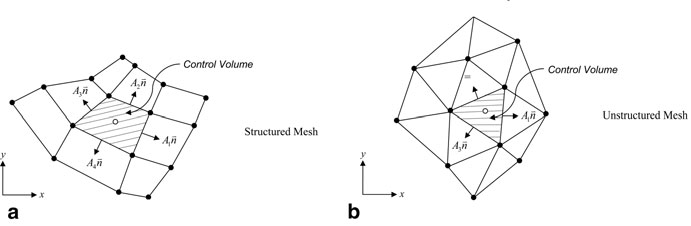
\includegraphics[width=\textwidth]{unstrfv}
  \caption{representation of mesh discretised with finite volume method}
  \label{usfv}
\end{figure}

Finite volume methods can tend to cause artificial, or numerical, diffusion if the mesh is of low quality. It is thus necessary to follow proper meshing practices, similar to those outlined in section \ref{Meshing}.

\subsection{Numerical Solution}

Once the system has been discretised, a system of linear equations can be developed to describe the system. These equations can be solved with one of several methods. These methods can generally be divided into two categories: either direct or iterative. In general, for large complex domains such as the nasal cavity models presented in this paper, iterative methods are the only way to derive a solution.

\section{Setup and solution of nasal cavity models used in this thesis}
Here an overview will be given of the way that the solution of the nasal cavity systems presented in this thesis will be given. Firstly the models are prepared and meshed as discussed in the Chapter \ref{MRM}. Once this is done the boundary conditions for the system must be defined. 

The face and internal wall of the nasal cavity and pipe extension are set to no slip condition. This means that velocity is assumed to be zero on the surface of these zones. The exit of the pipe extension is given a constant velocity value calculated for each model as to give an inspiritory flow rate of 10 lpm, which has been suggested by the literature to be a realistic approximation for an inspiratory rate of an adult human at rest. For these simulations this flow rate is treated as constant and the flow treated as steady, an assumption which greatly simplifies the solution process and one which is commonly used when comparing fluid flow characteristics between nasal cavity models (transient, or time dependant solutions are computationally much more costly). The 3D incompressible navier stokes equations were solved iteratively via the SIMPLE method for pressure-velocity coupling and a second order upwind scheme for convection.

The border of the hemispheric region around the face is set to atmospheric pressure. For resting inspiratory flow rates flow within the nasal cavity has been shown to be modelled most accurately as laminar; as such no turbulence model is used.

The temperature of the air coming from the outside is set to 20$^{\circ} C$ and the wall temperature inside the nasal cavity is set to 32.6$^{\circ} C$.  The species mass fraction of $\mathrm{H_2 O}$ to give 100\% relative humidity at the cavity wall is calculated for 32.6$^{\circ} C$, with the exception of the nasal vestibule, where diffusive flux is set to zero. The species mass fraction of $\mathrm{H_2 O}$ for the air coming into the model is calculated to give a relative humidity of 45\% for 101.3 kpa and 20$^{\circ} C$.

The numerical solution of the systems - described by the aforementioned boundary conditions and meshes - is approximated, for the models of this thesis, by the use of a commercial CFD code, in this case ANSYS FLUENT. The following chapter details the analysis of the solutions obtained for the five cavities.


\chapter{Results}

\section{Geometry Variations}
One-hundred cross-sectional slices were taken from the nostrils tip to the nasopharynx. From nostrils tip to choanae, vertical slices were made, while angled slices were made in the nasopharynx until the slice became horizontal (Figure \ref{fig:Slices}).

Figure \ref{fig:sil} shows 8 coronal slices taken at equidistant spacing across the sagittal axis between the anterior vestibule and the nasopharynx. We see the airway elongate vertically which increases the perimeter but maintaining a relatively constant surface area. This area to perimeter ratio has been cited as an important factor in the development of fluid flow in the nasal cavity. The thinner cavities also tend to exhibit higher wall shear stress. This is because of the steeper velocity gradients, which create stress through the viscosity of air, near the wall. This narrowness is also likely to influence heat and vapour transfer in the cavities; when the cavities are narrower there is less distance for the heat and vapour to travel from the wall to saturate the incoming air, and so it is likely to saturate the airflow more comprehensively. The variation in cavity thickness between the cavities can also be clearly observed in this figure.

Figure \ref{fig:area} shows the cross sectional area as a function of normalised distance along the sagittal axis. The distance has been normalised between the entrance to the nostrils and the end of the nasopharynx. A sample of cavities from the pre-existing literature has also been included for comparison. A significant variation can be seen in the average cross sectional area of the models presented in this paper; This variation is most pronounced towards the rear of the cavities. None of the models show quite the same volume as the atrophic rhinitis model, also shown here as Garcia prior to the nasopharynx, although the 64yo is close. The general shape of the curve is reasonably similar for the various models in this paper, with notable exceptions in the Nasopharynx of the 64yo cavity and a larger spike in the vestibule region of the 78yo. Observations from Figure 3 can be compared with the cross sectional silhouettes from Figure 2, for a clearer understanding of the variations in geometry between the 4 models presented here. The range of cross-sectional areas allows us to observe the relationship between various fluid mechanical properties of the cavity and cavity volume/cross-sectional area.

Table \ref{tab:secvol} - \ref{tab:deff} shows the variation of the volume, surface area and effective diameter respectively, in comparison with models from the literature. The volumes of the four models presented in this paper varied significantly. The largest discrepancies were noted in the pharynx and turbinate regions, with a less marked discrepancy in the vestibular region. The 48 – yo is showing greater volume than that seen in the atrophic rhinitis patient from \cite{Garcia2007}. The surface area of the atrophic rhinitis model is also significantly lower, to the extent that the effective diameter, shown in Table \ref{tab:deff}, is larger than the models presented in this paper.

Minimal cross sectional area, shown in Table \ref{tab:mca}, is significant to flow across the cavity\cite{Lindemann2008}. Here the atrophic rhinitis model shows larger minimal cross sectional area than any of those found in the models presented here, although it is quite close to that of the 64yo.

The circularity shape factor (a dimensionless quantity used in image analysis) was used to quantify the cross-sectional shape (Figure \ref{fig:Circ}). The circularity, $f_o$ , (also known as the isoperimetric quotient), is the ratio of cross-sectional area bounded by a closed curve, to its perimeter defined as, 

$ f_o = \frac{4 \pi A}{P^2} $

At the nostril inlet, the circularity ranges from 0.18-0.30 and this reduces to a value of approximately = 0.035 (except the 64yo model). It then increases rapidly towards 1 where the two nasal chambers merge and form a single conduit in the form of the nasopharynx.

\begin{figure} \label{fig:geo}
  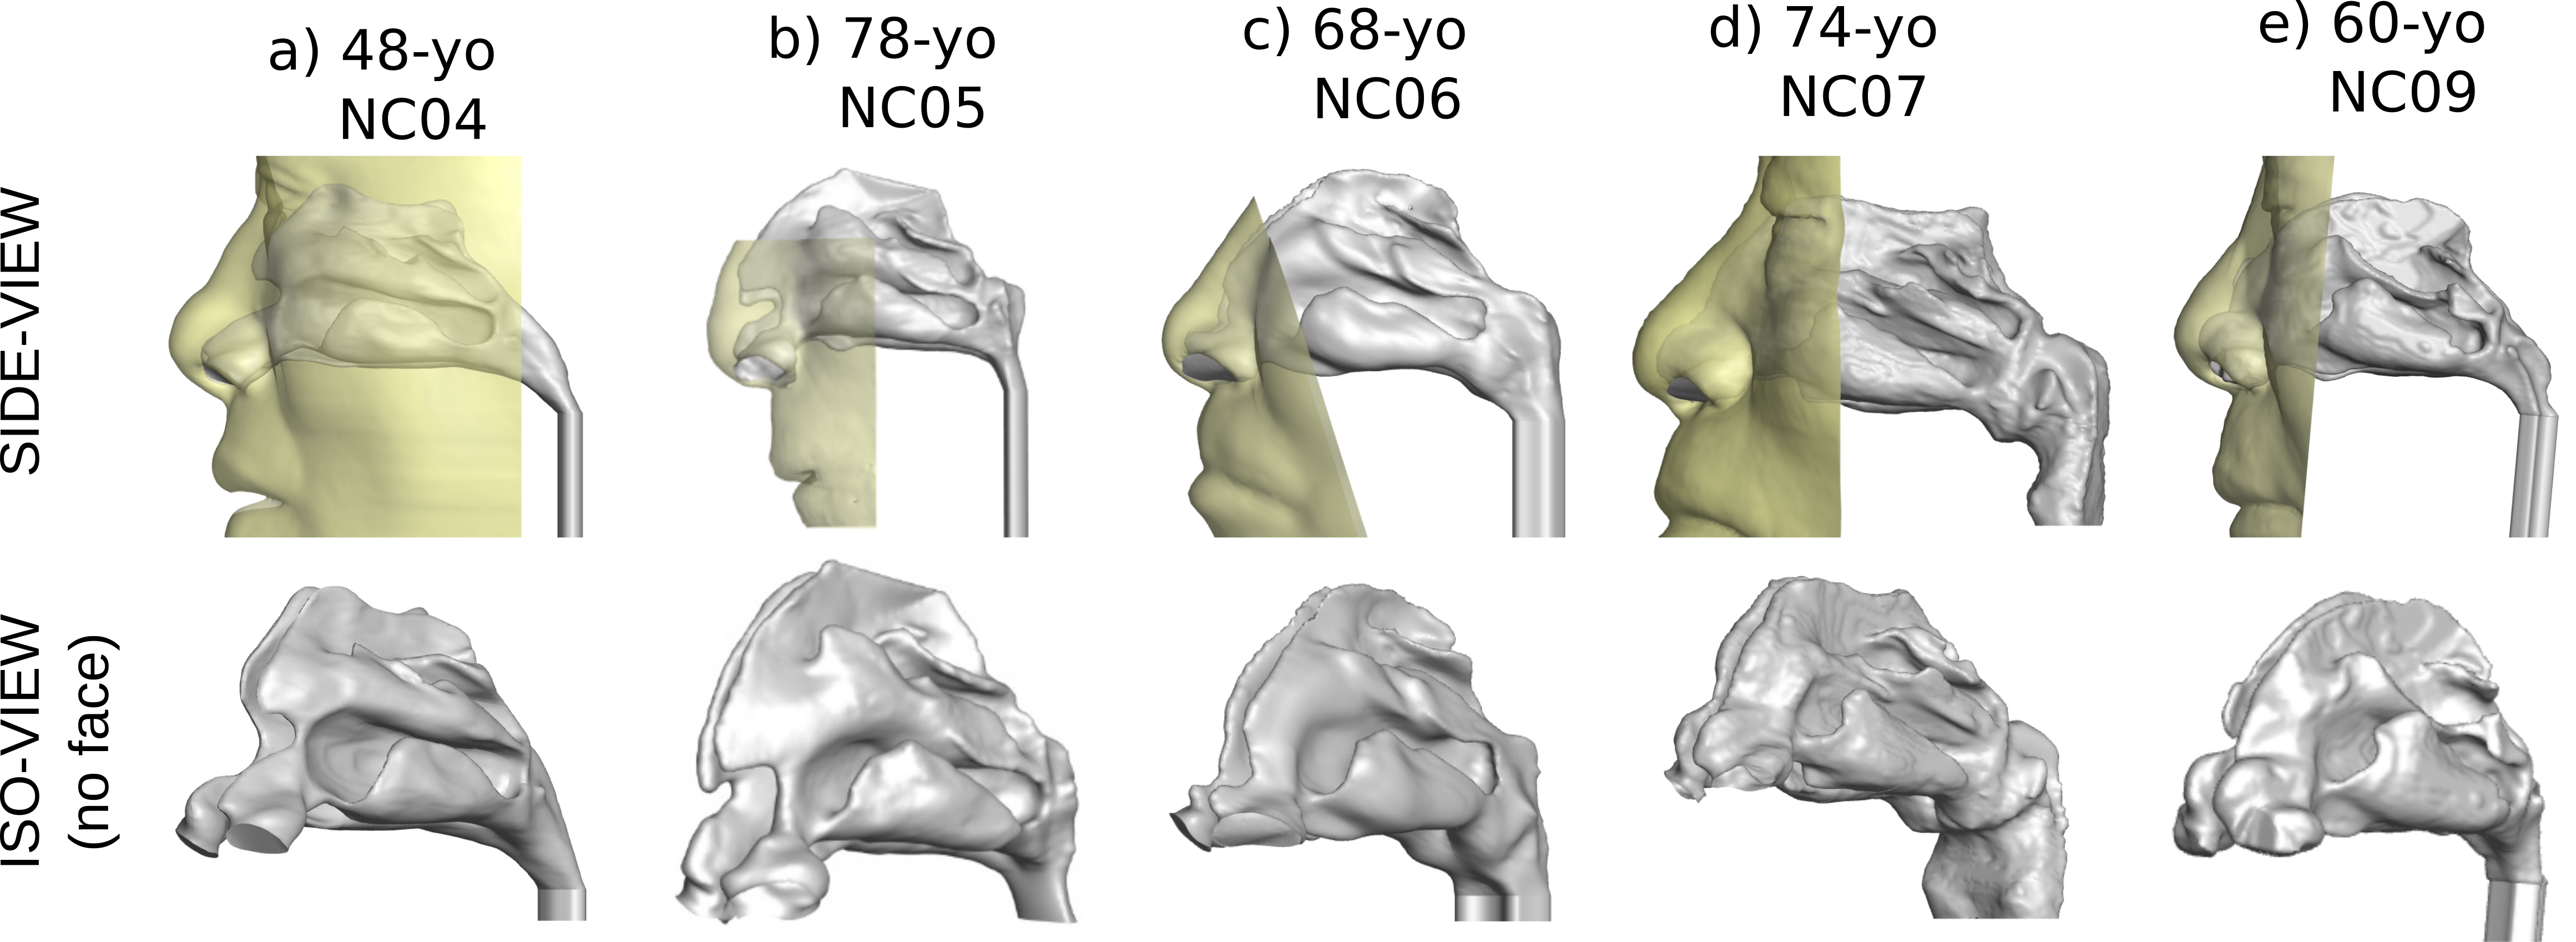
\includegraphics[width=\textwidth]{geometries}
  \caption{geometries of the five cavities}
\end{figure}

\begin{figure} 
  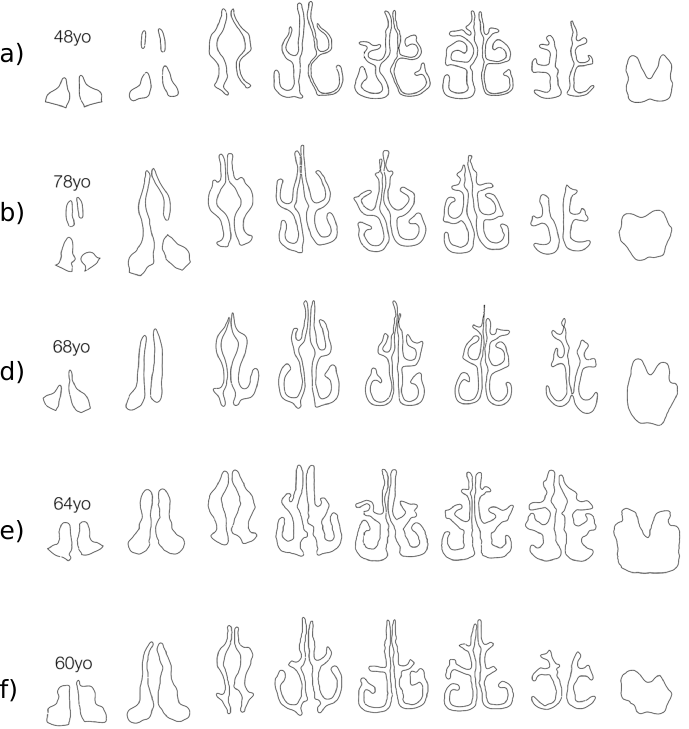
\includegraphics[width=\textwidth]{Silhouettes}
  \caption{silhouettes of the cavities}
  \label{fig:sil}

\end{figure}

\begin{figure}
\centering
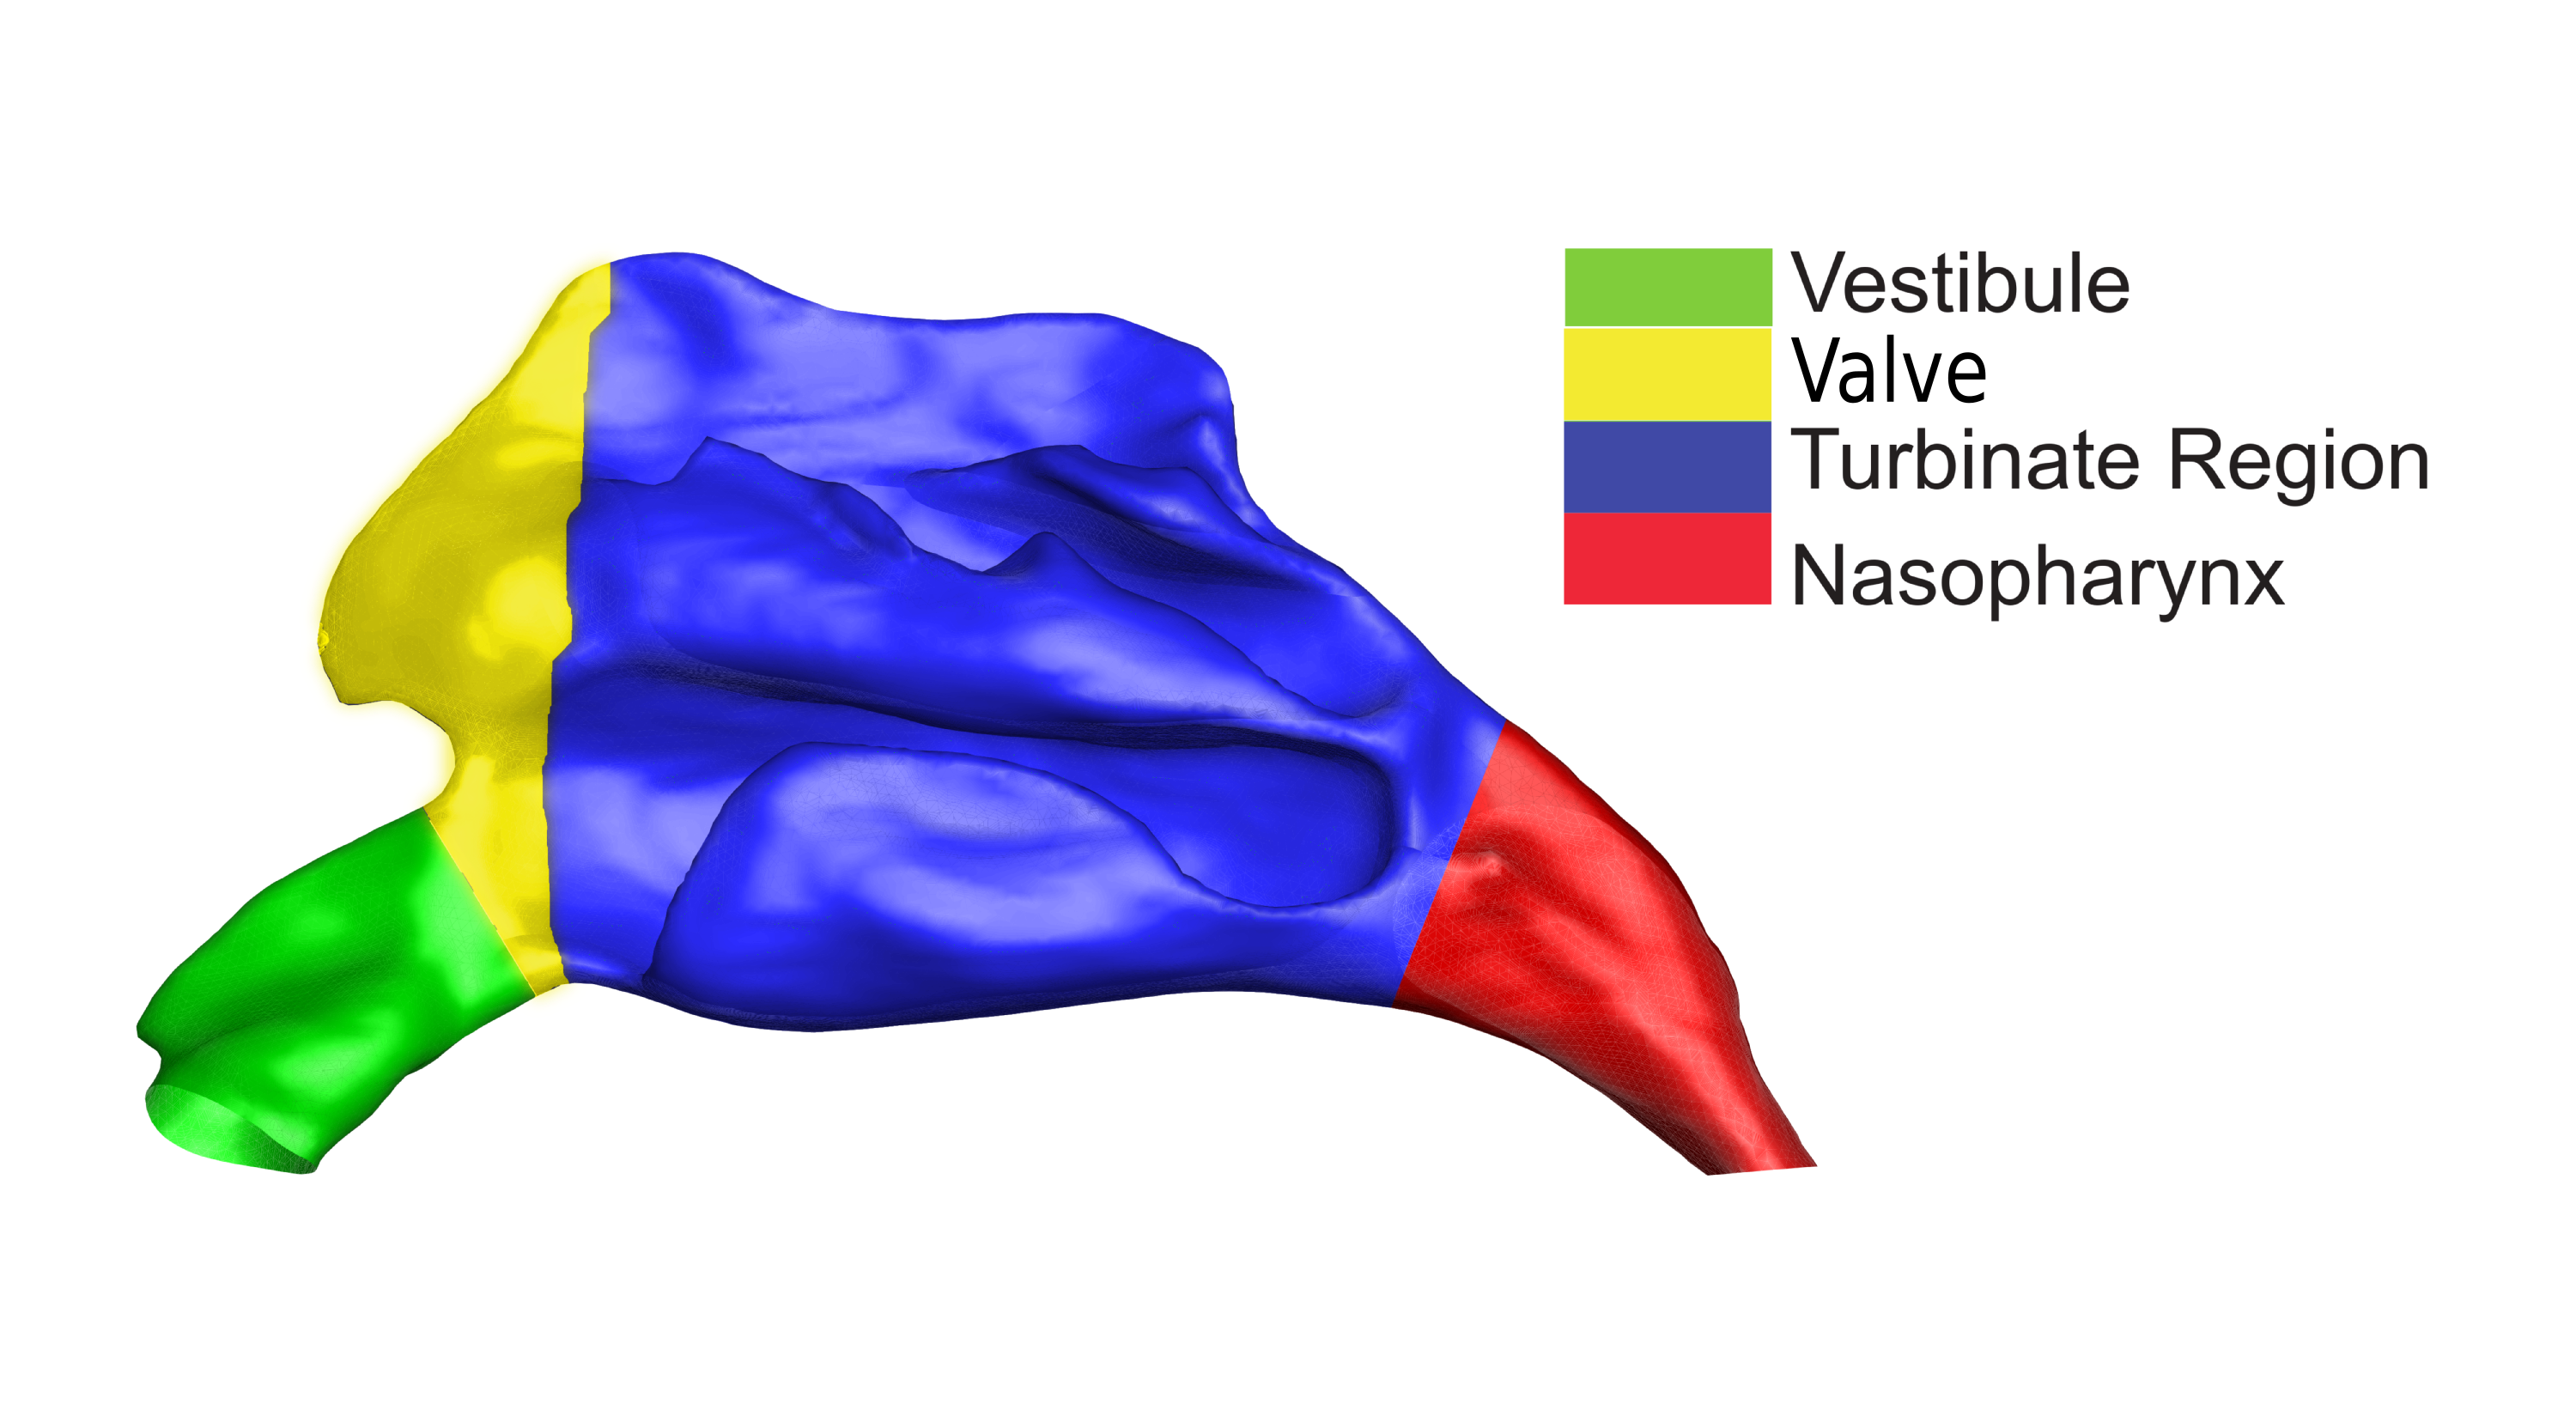
\includegraphics[width=0.7\textwidth]{regions}
\caption{Colour coded display of the regional divisions used in tables \ref{tab:secvol}, \ref{tab:secsa}, \ref{tab:deff}} 
\label{fig:regions}
\end{figure} 

\begin{figure} 
\centering
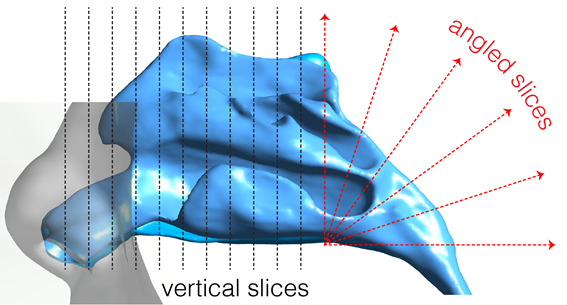
\includegraphics[width=0.7\textwidth]{slicesSchematic}
\caption{Representation of the slicing method used for sampling data across the sagittal axis throughout this thesis} 
\label{fig:Slices}
\end{figure}

\begin{figure}
  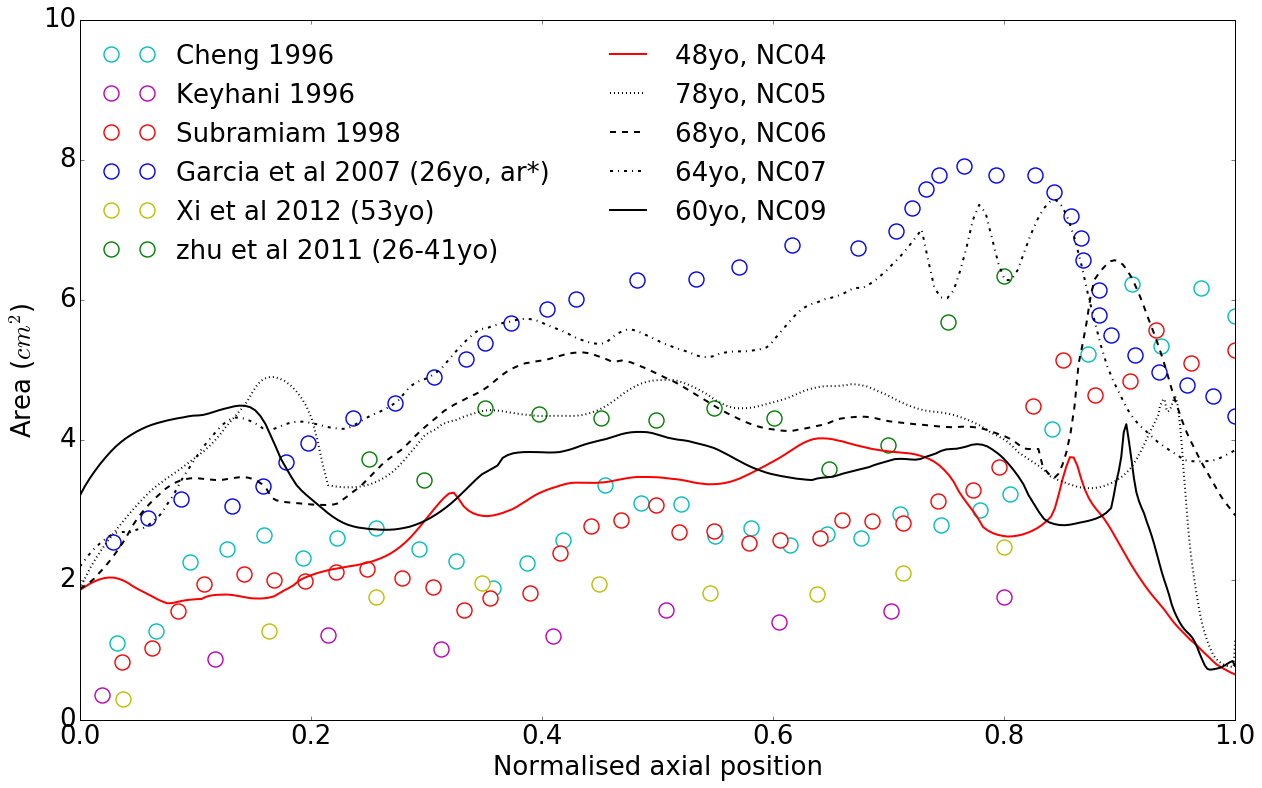
\includegraphics[width=\textwidth]{Areavsdistance}
  \caption{area versus distance across the four nasal cavities with a series of examples from the literature}
  \label{fig:area}
\end{figure}

\begin{figure}
\centering
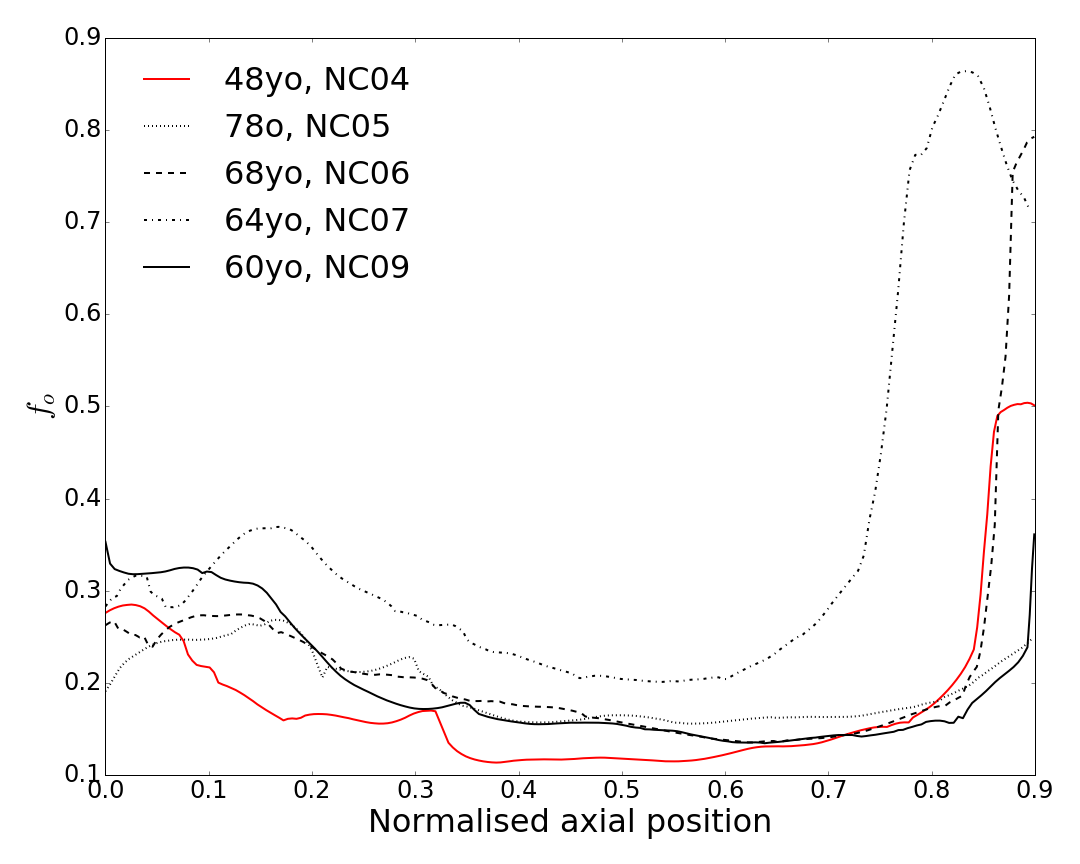
\includegraphics[width=1\textwidth]{circularity}
\caption{area to perimeter ratio variation with normalised length of the nasal cavity from the nostril inlet to the nasopharynx. This length for each model is: 48yo – 8.97cm; 60yo – 9.26cm; 64yo – 9.60cm; 68yo – 9.31cm; 78yo – 8.45cm}
\label{fig:Circ}
\end{figure}
\begin{table}
  \begin{tabular}{p{0.125\textwidth}p{0.1\textwidth}p{0.1\textwidth}p{0.1\textwidth}p{0.1\textwidth}p{0.1\textwidth}p{0.11\textwidth}p{0.13\textwidth}}
 & \textbf{48yo} & \textbf{78yo} & \textbf{68yo} & \textbf{64yo} & \textbf{60yo} &\textbf{Xi et al. \cite{Xi2012}} & \textbf{Garcia et al.\cite{Garcia2007}} \\
\cline{2-8}
\textbf{Turbinal region} & 18.54 & 22.78 & 24.62 & 30.722 & 16.73 & 12.63 & 33.66\\
\textbf{Naso-pharynx}  & 3.84 & 5.40 & 12.80 & 20.09 & 4.57 & 16.33 & 10.60\\
\textbf{Vestibule} & 3.10 & 4.15 & 2.81 & 4.21 & 7.39 & 5.50 & 2.41\\
\textbf{Total} & 25.48 & 32.33 & 40.23 & 55.07 & 28.69 & 34.43 & 47.77 \\
\hline
\end{tabular}
\caption{ sectional volume, according to sections as seen in Figure \ref{fig:regions} ($ cm^3 $)}\label{tab:secvol}
  \begin{tabular}{p{0.125\textwidth}p{0.1\textwidth}p{0.1\textwidth}p{0.1\textwidth}p{0.1\textwidth}p{0.1\textwidth}p{0.11\textwidth}p{0.13\textwidth}}
 & \textbf{48yo} & \textbf{78yo} & \textbf{68yo} & \textbf{64yo} &\textbf{60yo}& \textbf{Xi et al.} & \textbf{Garcia et al.}\\
 \cline{2-8}
\textbf{Turbinal region} & 170.92 & 174.07& 190.44 & 163.44 & 138.80 & 112.59 & 133.50\footnote{includes vestibule} \\
\textbf{Naso-pharynx} & 12.20 & 12.80 & 25.23 & 40.42 & 11.37 & 40.93 & 31.46\\
\textbf{vestibule} & 15.71 & 17.37 & 12.45 & 17.92 & 46.96 & 35.58 &  -\\
\textbf{total} & 198.82 & 204.25 & 228.11 & 221.79 & 197.192 & 189.10 & 164.96\\
\hline
\end{tabular}
\caption{sectional surface area, according to sections shown in Figure \ref{fig:regions}($ cm^2 $)}\label{tab:secsa}
  \begin{tabular}{p{0.125\textwidth}p{0.1\textwidth}p{0.1\textwidth}p{0.1\textwidth}p{0.1\textwidth}p{0.1\textwidth}p{0.11\textwidth}p{0.13\textwidth}}
& \textbf{48yo}  & \textbf{78yo} & \textbf{68yo} & \textbf{64yo} & \textbf{60yo} & \textbf{Xi et al.} & \textbf{Garcia et al.}\\
 \cline{2-8}
\textbf{Turbinal region} & 0.434 & 0.52 & 0.52 & 0.75 & 0.48 & 0.45 & 1.11\\
\textbf{Naso-pharynx} & 1.26 & 1.69 & 2.03 & 1.99 & 1.61 & 1.60 & 1.35\\
\textbf{vestibule} & 0.79 & 0.96 & 0.90 & 0.94 & 0.63 & 0.62 &  - \\
\textbf{total} & 0.51 & 0.63 & 0.71 & 0.99 & 0.58 & 0.72 & 1.13 \\
\hline
\end{tabular}
\caption{Effective diameter $d_{eff} = \frac{4v}{a} (cm) $}\label{tab:deff}

  \begin{tabular}{p{0.125\textwidth}p{0.1\textwidth}p{0.1\textwidth}p{0.1\textwidth}p{0.1\textwidth}p{0.1\textwidth}p{0.11\textwidth}p{0.13\textwidth}}
& \textbf{48yo}  & \textbf{78yo} & \textbf{68yo} & \textbf{64yo} & \textbf{60yo} & \textbf{Xi et al.} & \textbf{Garcia et al.}\\
 \cline{2-8}
 \textbf{MCA}&1.665&3.0174&1.80&4.14&2.7&Unknown&3.04
\end{tabular}
 \caption{Minimal axial cross sectional area $(cm^2)$}\label{tab:mca}
\end{table}
\section{Pressure Drop}

The pressure drops across the nasal cavities can also be seen in Figure \ref{fig:stpr} to vary in relation to the volume of the nasal cavity. This is in contrast to the experimental findings of \cite{Lindemann2008, Edelstein1996, WhanKim2007}, who’s studies using rhinomanometry showed no significant decrease in pressure across the cavity to accompany the recorded variation in volume. The cause of this discrepancy is unclear. Here the pressure drop is primarily seen across the valve region. Here the nasopharynx has been excluded from the domain; the significant pressure drop across the nasopharynx was inversely proportional to the cross sectional areas of the respective nasal cavities

The pressure drops can be seen in Figure \ref{tab:pvv} to decrease in relation to the volume of the cavity. This fits well with the findings of previous experimental studies looking at pressure drops across nasal cavity models, as can be seen from the comparison with results from \cite{Garcia2007} and \cite{Kelly2004}, both displayed in figure \ref{tab:pvv}.

  \begin{table} 
    \centering
  \pgfplotstableset{
  every head row/.style={before row=\toprule,after row=\midrule},
  every last row/.style={after row=\bottomrule}}

  \pgfplotstabletypeset[
      fixed zerofill,
      precision=2,
      display columns/0/.style={string type},
      col sep=comma]{tables/prvsflow.txt}
  \caption{Variation of pressure drop with flow rate (m/s)}
  \label{tab:pvv}
\end{table}

\begin{figure} 
  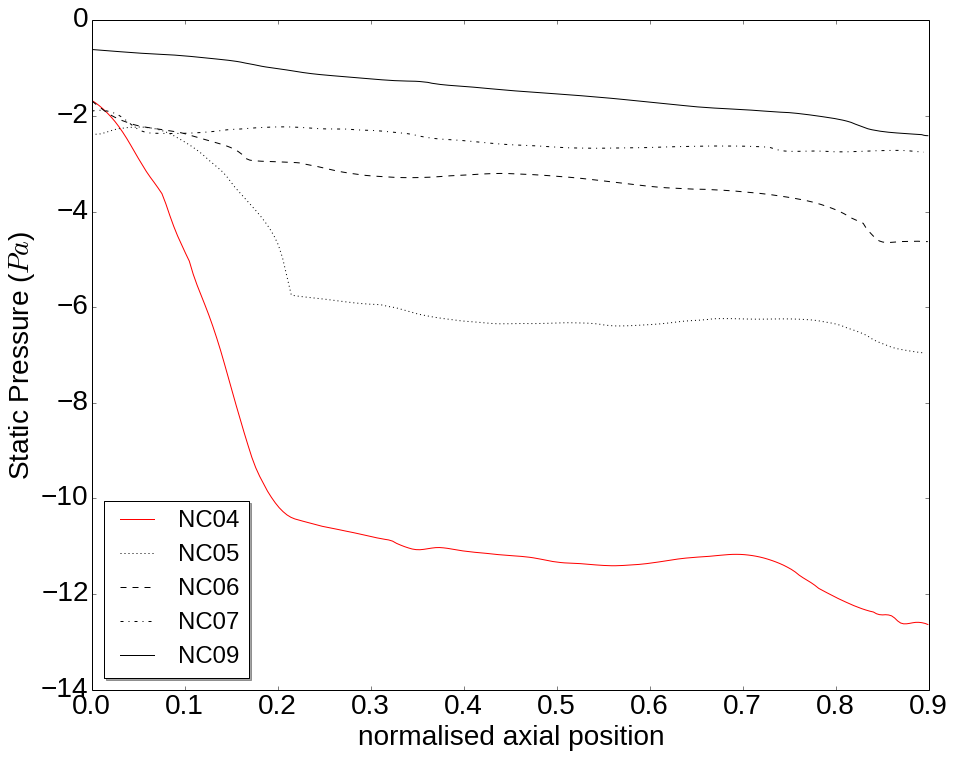
\includegraphics[width=\textwidth]{statpres}
  \caption{area versus distance across the four nasal cavities with a series of examples from the literature}
  \label{fig:stpr}
\end{figure}

\section{Wall Shear Stress and velocity}
Figure \ref{fig:vsl} shows flow streamlines through the left and right nasal chambers with the chamber’s wall shear stress. In all the models flow acceleration and high wall shear stresses were consistently found in the region between the nasal vestibule entrance (anterior) and before the middle nasal passage. We also note that there is a preference for the streamlines to pass through the mid-height of the nasal chambers. A small fraction reached the olfactory region, and some inferiorly along the floor of the chambers. The highest wall shear stress values were found in the 48yo, 60yo, and 78yo models which are also the models with the smaller cross-sectional area profiles (from Figure \ref{fig:area}), and corresponds to the highest velocity magnitudes produced by the streamlines in the models. Wall shear stress contours viewed from the top and lateral left-chamber side of all nasal models are shown in Figure \ref{fig:wcont}. By using the same colour scale the results show directly the disparity between nasal models.

Figure \ref{fig:wcont} shows the wall shear stress across the five models presented in this paper. The valve region can be seen to be a region of particularly high wall shear across all the models. Also note that the locations of high wall shear vary significantly in the more voluminous cavities


From Figure \ref{fig:wax}, Wall shear stress can be seen to be more pronounced in general in the more voluminous models such as the 48yo, and in particular this effect is exaggerated in the valve region. Here the wall shear stress is mapped rom the nostrils to the entrance to the nasopharynx. The nasopharynx showed more pronounced variations, in particular the 48yo showed a significant spike in wall shear stress in the nasopharynx, which is to be expected because of its lower cross sectional area. Note that the sagittal distribution of wall shear stress is much more even in the larger cavities.  The valve region - considered of particular significance to the development of flow features within the nasal cavity \cite{Lindemann2008} – shows significant variation in wall shear stress concentration, with the 64yo and 60yo presenting a very even distribution of wall shear stress, in contrast to the 48yo or 78yo which show wall shear more pronounced around the opening from the vestibule. Similar variations can also be seen in the distribution within the turbinal region (Figure \ref{fig:wcont}). 

Cross-sections at the internal nasal valve, and turbinate region were taken for each model and its velocity contour presented in Figure \ref{fig:wcs}. We traced the perimeter of each cross-section starting from its apex and follow down in a counter-clockwise direction. For the nasal valve cross-section in all models, we found that the surface proportion was distributed almost evenly between the lateral and septum walls, since its partition occurred at 0.5. For the turbinate region, this value was 0.7 meaning that 70\% of the perimeter resides along the lateral side and 30\% of the perimeter is along the septum wall. For the 48yo model we labelled three peaks for the nasal valve slices (r1, r2, and l1) to help identify the locations on the cross-section itself. 

Wall shear stress peaks occurred close to the regions of maximum velocities in the contours. Superiorly, where the velocity is very low, the wall shear stress is nearly zero. These peaks and troughs correlate well with the contour slices and is consistent for all models.

\begin{figure} 
  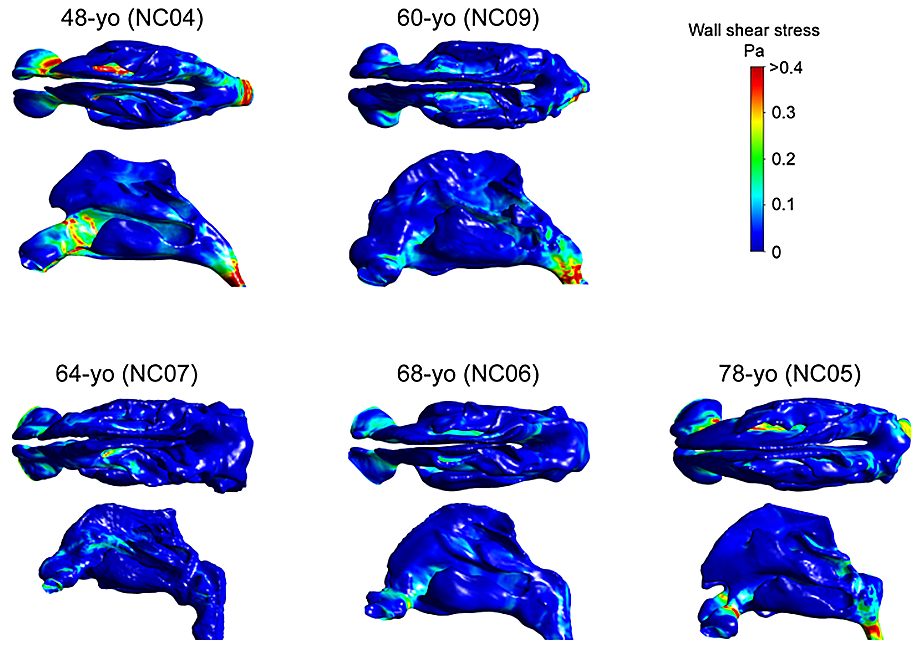
\includegraphics[width=\textwidth]{wsscont}
  \caption{Direct comparison of WSS surface contours between all models}
    \label{fig:wcont}
\end{figure}

\begin{figure} 
  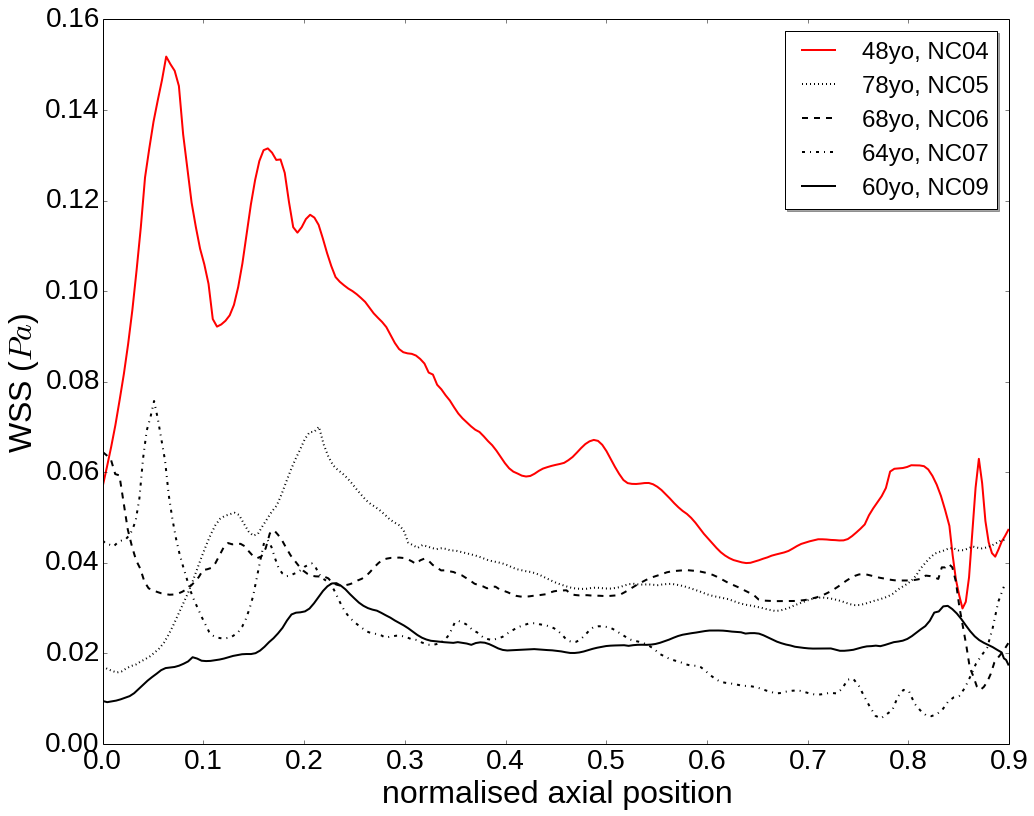
\includegraphics[width=\textwidth]{axialwss}
  \caption{coronal area weighted average of wall shear stress plotted as a function of distance from the entrance to the cavity across the saggital axis}
  \label{fig:wax}
\end{figure}

\begin{figure} 
  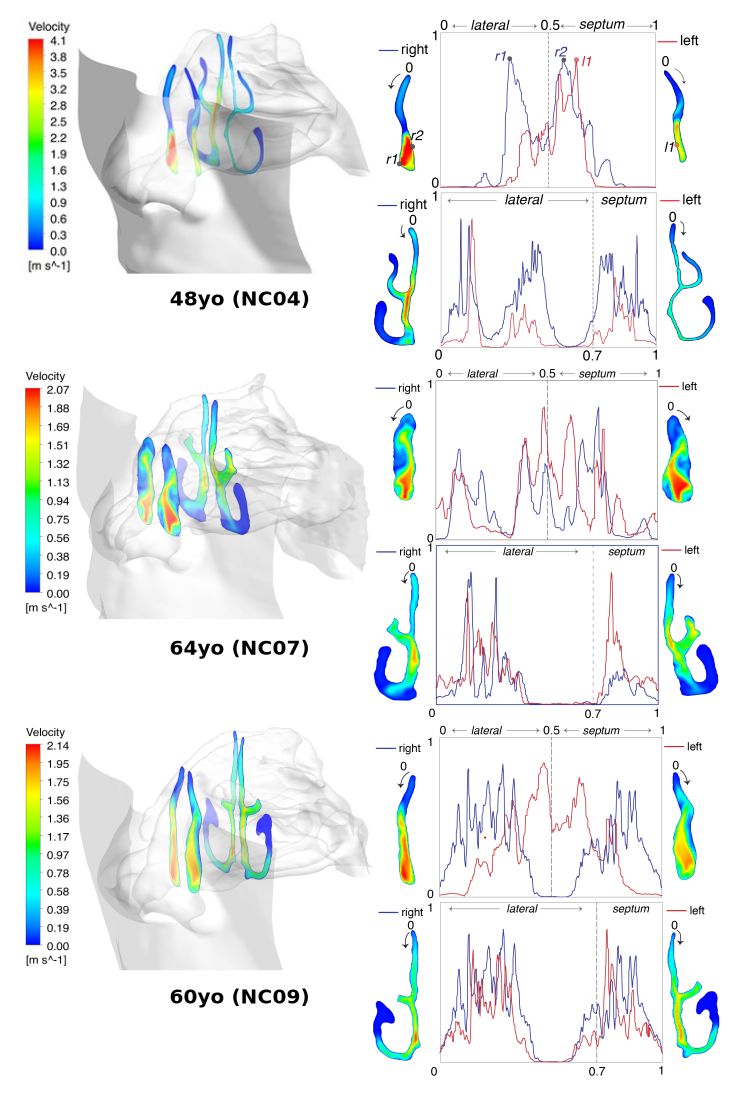
\includegraphics[width=\textwidth]{wsscs/wsscs1}
  \label{fig:wcs}
\end{figure}

\begin{figure} 
  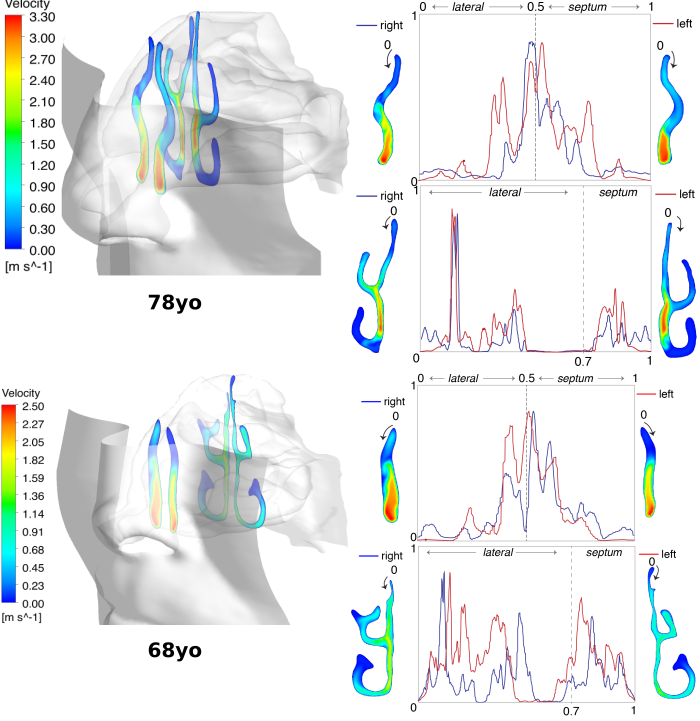
\includegraphics[width=\textwidth]{wsscs/wsscs2}
  \caption{Velocity contours and wall shear stress values along the perimeter outlines of two cross-sections. The x-axis is the perimeter distance starting from the top apex of each cross-section slice, and moves along the perimeter laterally. One full tracing around the perimeter is defined as 1.0. The dashed line represents the floor of the cross-section opposing its apex, and for the nasal valve, the halfway point \(0.5\), while for the turbinate cross-section it is 0.7. The y-axis represents normalized wall shear stress \(0 - 1\).}
  \label{fig:wcs}
\end{figure}

\begin{figure} 
  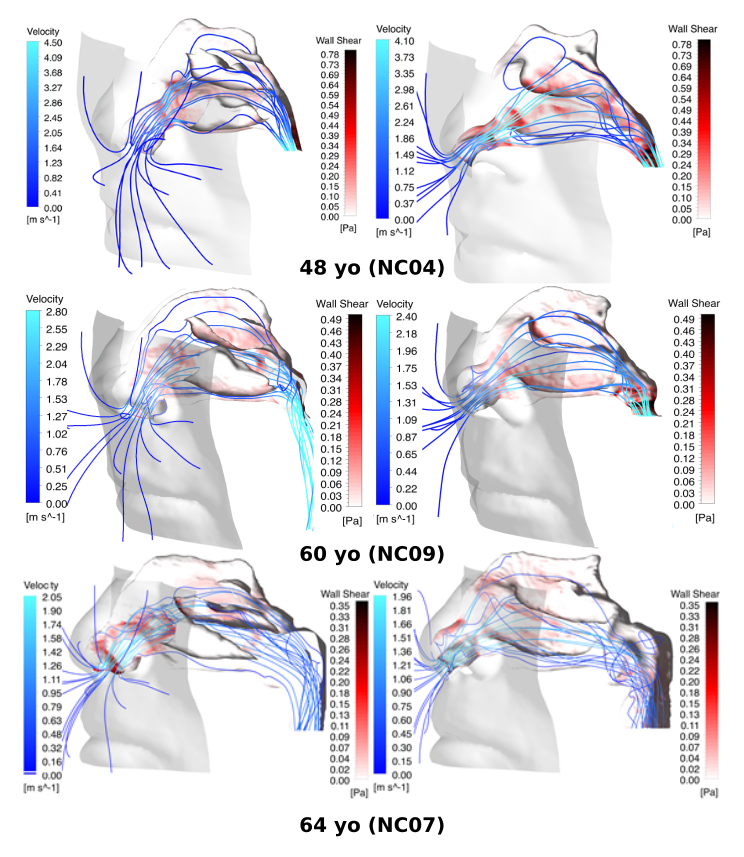
\includegraphics[width=\textwidth]{streamlines/sl1}
  \end{figure}

\begin{figure} 
  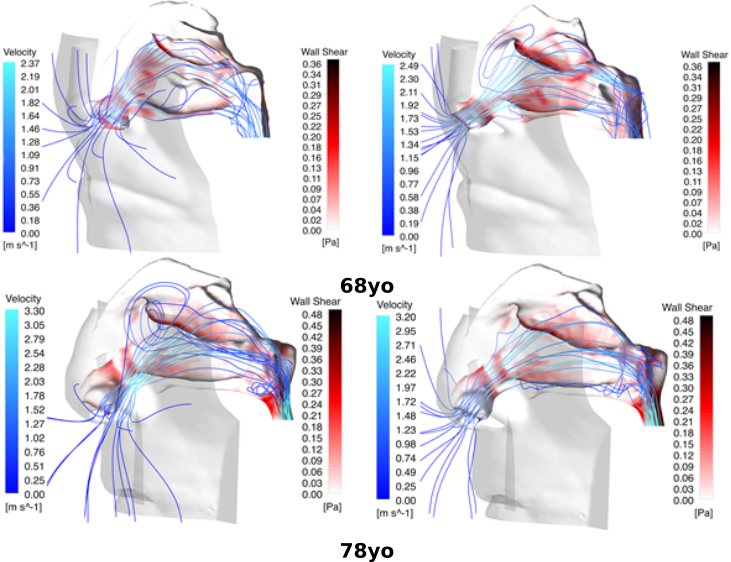
\includegraphics[width=\textwidth]{streamlines/sl2}
  \caption{Flow streamlines (coloured in blue) passing through the left and right chambers of the nasal cavity. Each chamber’s wall shear stress is shown (coloured in red).}
  \label{fig:vsl}
\end{figure}

 
\section{Heat and Vapour Transfer}

Some variation in the heat and vapour transfer efficacy can be seen between the models presented in this thesis. Note the higher than average figures for temperature and h2o mass fraction in the valve area of the 78yo. In general the more voluminous models exhibit lower humidity and temperature (Figures \ref{fig:h2o} and \ref{fig:Temp}). The data from the atrophic rhinitis study by Garcia et al \cite{Garcia2007}; the humidity and temperature distribution in this model seem to be lower in proportion to the increased voluminousness of this model (see figure \ref{fig:area}).

\begin{figure} 
  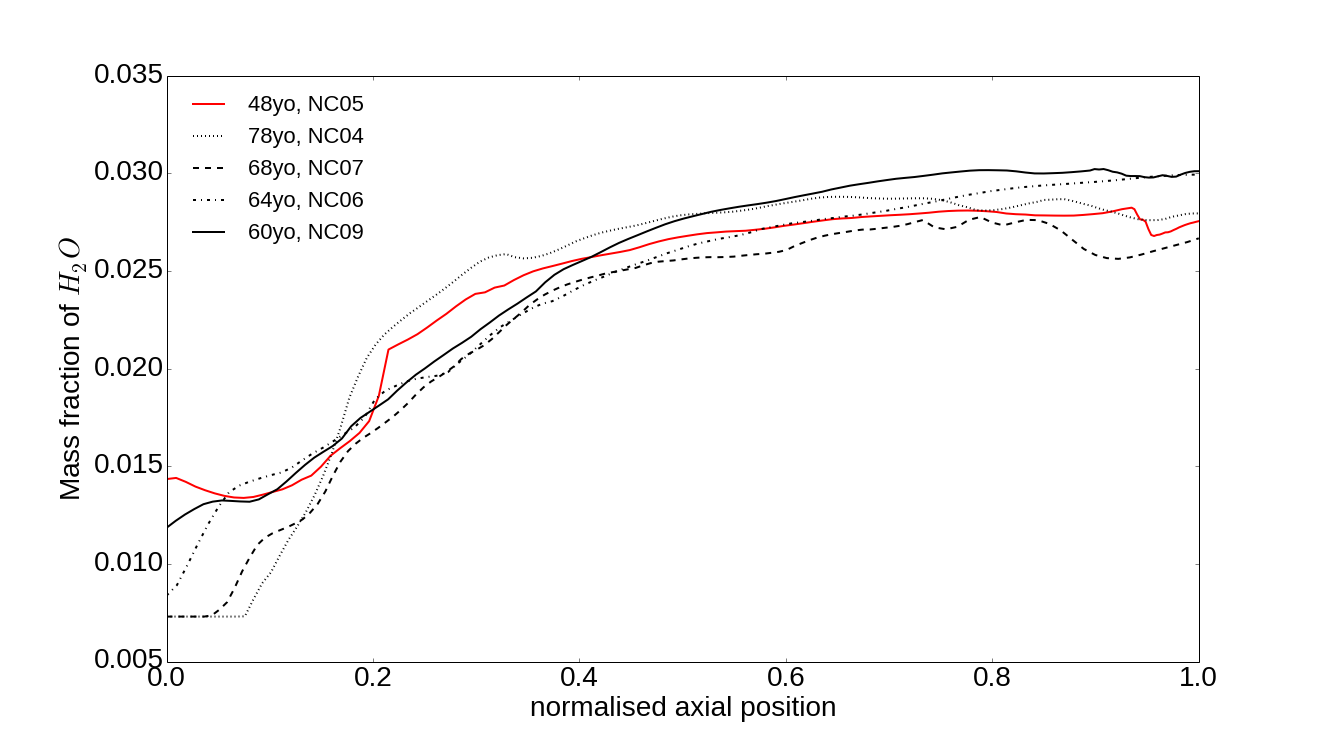
\includegraphics[width=\textwidth]{h2o}
  \caption{average mass fraction of h2o as a function of normalised saggital position}
  \label{fig:h2o}
\end{figure}


\begin{figure} 
  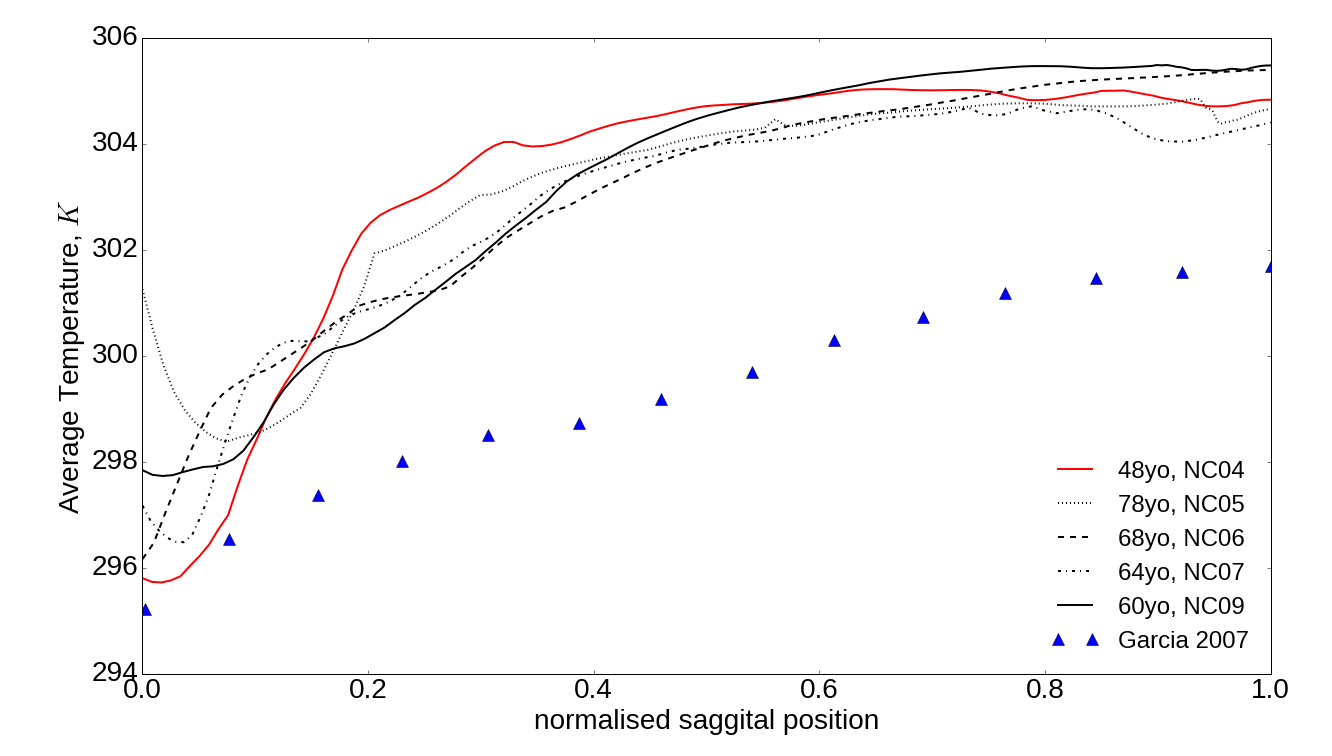
\includegraphics[width=\textwidth]{Temperature}
  \caption{average ambient temperature as a function of normalised saggital position}
  \label{fig:Temp}
\end{figure}


\chapter{Discussion}

Evaluation of nasal respiratory function for diagnostic or research purposes relies on categorisation of an individual's demographics, including age, gender, and ethnicity. It is known that normal changes in inter- or intra-individual nasal cavities manifest through age. This is especially true of intranasal volume, which is thought to increase due to hormonal changes leading to mucosal atrophy\cite{Kalmovich2005, Lindemann2010}. Edelstein\cite{Edelstein1996}  and Lindemann et al.\cite{Lindemann2008}  found correlations between aging and the occurrence of a range of rhinological conditions (e.g. dry cold itchy noses; crusting, postnasal dripping and obstructed nasal breathing) although their association with nasal morphology was not established. Thus, a detailed analysis of the nasal morphology and its effect on respiratory function in older adult patients may contribute towards this understanding.

Demographic factors such as age, gender, and ethnicity play an important role in
determining one’s nasal anatomy and physiology. For example, it was found that males exhibited larger nasal cavities e.g. larger normal pharyngeal areas in males over females\cite{Huang1998, BROOKS1992}. However, very few studies have quantified these differences. In terms of geographic variations with age, Kalmovich, et al.\cite{Kalmovich2005} found a significant increase in nasal cavity volume and minimal cross sectional area with age using acoustic rhinometry on 165 patients. Later, Lindemann, et al.\cite{Lindemann2010} used acoustic rhinometry in conjunction with rhinomanometry and validated questionnaires to survey the nasal cavities of eighty patients. While the questionnaire and rhinomanometry did not show any difference between the older and younger subjects, a marked increase in the volume of the nasal cavity with age was found from the acoustic rhinometry data. More recently, Loftus, et al.\cite{Loftus2016}  found higher intranasal volumes with age on CT volumetric analysis.

In the past, quantifying differences in nasal airflow has been limited by a lack of sensitive tools that can quantify the complexities of the sinonasal cavity. More recently, CFD has been proven to be a useful tool for detailed analysis of nasal airflow. With this new tool, normative data based on demographics is required so that these can be compared with disease states. We aimed at investigating the nasal airflow anatomy and physiology of older Chinese adult males to understand geometry features and dynamics of inhaled flow field in this specific demographic group.

Our geometry analyses revealed the significant influence of the area to perimeter ratio on fluid flow development in the nasal cavity. The thinner cavities exhibited higher wall shear stresses due to sharper velocity gradients that were produced. The narrow geometry would also increase heat and vapour transfer as there is less distance for the heat energy and vapour to transport from the wall to condition the inhaled air.

The cross-sectional area of slices taken along the nasal cavity, provided insight into the patient’s airway patency based on the degree of openness of the nasal chamber. These observations (from Figure \ref{fig:area}) can be compared with cross sectional outlines in Figure \ref{fig:sil} which allow predictions of the likely relationships between fluid flow properties caused by the individual nasal geometry features.

A shape factor in the form of the circularity,   described the overall shape of each cross-sectional slice along the nasal cavity geometry. A circularity of 1 implies a circular shape, although this can be masked by irregular shapes that coincidently have the same values as a smooth circle. A value close to zero, however is more definite providing a strong suggestion of a jagged and non-circular shape. The sharp increase in the circularity plot indicated where merging of the two chambers occurs. The circularity is a well-established measurement commonly used in image analysis of particles, and this is the first time it has been applied for shape detection in nasal cavity geometries. The results in this study showed that circularity is useful as an indicator and quantifiable metric for identifying the anterior, middle, and posterior nasal cavity regions.

Fluid flow analysis showed the relationship between inhaled fluid dynamics and its impact on nasal sensation in the form of fluid-surface shear. Regions of high acceleration were often caused by the airway converging into a smaller cross-section thereby accelerating the flow through.  This corresponded with a high wall shear stress region in the vicinity of the minimised cross-section. The results showed that the middle region partition in this study incorporated the minimum cross-sectional area into its region, which is known to occur around the nasal valve, although it could be considered as part of the anterior nasal cavity.

The 48yo and 60yo models were the smallest in size and this resulted in higher wall shear stress magnitudes. Based on the geometry analysis, peak velocities and wall shear stresses should occur at the minimal cross-sections, and this corroborated well with the highest values indeed found in the 48yo and 60yo models. Locally, the highest wall shear stress concentrations occurred around the internal nasal valve, and this is consistent across all the models. Interestingly the nasopharynx also exhibited a significant increase in wall shear stress, and this was due to the cross-sectional area decreasing at the nasopharynx.

The wall shear stress profiles along cross-sectional slices showed peak wall shear stresses produced inferiorly on the internal nasal valve while there was very low wall shear stresses superiorly. For the turbinate slices, the velocity contours showed the bulk flow and peak velocity were offset from the nasal floor. This is the continuation of the fluid flow that was rising from the nasal valve region. The main nasal passage expands but the flow is unable to reach the new extremities.

The static pressure variation shown in Figure \ref{fig:stpr} merits some discussion. Although it would seem logical that an increased cavity volume would have the effect of reducing pressure drop, this is not the result that has been recorded by previous researchers using rhinomanometry \cite{Lindemann2008}. This discrepancy is possibly due to the flexibility of the nasopharynx, varying the diameter of the exit in ways that are not replicated in the ct models.

The more even distribution of wall shear stress - both sagittally, as seen in Figures \ref{fig:wcont} and \ref{fig:wax}; and coronally, as seen in Figure \ref{fig:wcs} - is indicative of variations in airflow structure and therefore performance of the nasal cavity models. In particular the variation in the local maxima for WSS found in the region of the nasal valve is indicative of varying air conditioning capacity.

It seems in particular that it is only in the more severely enlarged cavities that drastically increased vorticity is seen in the air flow structures. The volume of the NC07 model of 55.07 $cm^3$.

It seems probable that these marked increases in vorticity are linked to the observed reductions in air-conditioning functionality in specimens from this age group \cite{Lindemann2009a}. This is in accordance with the findings of \cite{Garcia2007} in relation to atrophic rhinitis patients. The model in their study had a recorded volume of 34.5 $cm^3$, however this was only measured to the end of the septum, and a comparison with the models from this study, as seen in Figure ~\ref{fig:area} shows that the volume through the turbinal region of the atrophic rhinitis model was significantly larger than that of the largest model from this study, NC07. Although a quantity is not given for the volume of the nasopharynx in the atrophic rhinitis model, qualitative comparison between the  images of the model and those of the models from this study seem to show that the significant expansion of the nasopharynx which is present in all of the elderly models was not present in the model of the younger (26 yo) atrophic rhinitis sufferer. 

previous research has suggested that the presence of significant vortices such as those seen in the larger of the models presented in this study is related to the impairment of air conditioning functionality. The specifics of this mechanism , however, are yet to be investigated, and this is a piece of work which should be completed in future. In addition, the impact of the observed variations in airflow structure on the ability of the nasal cavity to filter particles from the air has not been investigated, and this is also an area which could be of some significance.

The heat and vapour transfer figures show what seems to be close to an inverse linear relationship between the voluminousness of the cavities and their heat and vapour transfer efficacy. This is particularly pronounced in the nasal valve. This relationship agrees well with the data from Garcia et al \cite{Garcia2007} taken from their atrophic rhinitis patient. This suggests that the mechanisms causing this reduced efficacy in the atrophic rhinitis patient are the same as those in elderly patients; this may imply that, for more extreme cases, that the surgical procedures implemented for atrophic rhinitis patients could also be effective for the elderly. It has been suggested by \cite{Lindemann2008} that heat and vapour transfer are significantly effected by the minimal cross sectional area. The current data doesn't show anything to support or disprove this suggestion, as in general the models presenting higher mcas are also presenting higher voluminousness. In fact, the model that shows the highest MCA relative to its voluminousness [NC09], shows very good heat and vapour transfer.

Detailed understanding of the associations among variabilities in nasal anatomy, age, and airflow dynamics will greatly improve current knowledge regarding the influence of conductive mechanisms on olfactory ability. Variabilities in nasal 
anatomy have traditionally been understood to influence olfaction\cite{Eiting2015, Craven2007}. Nasal profiles that have been postulated to be associated with improved olfaction include the dorsal conduit, which delivers inhaled odorant-laden air to the olfaction recess through enhanced olfactory airflow, and an enlarged olfactory recess at the posterior end of the nasal cavity\cite{Eiting2015, Craven2007, Eiting2014}. It has also been reported that anatomical changes in the olfactory cleft or the nasal valve region alter odorant transport to the olfactory epithelium\cite{Zhao2004a}. Furthermore, the incidence of olfactory dysfunction in the general population is unclear, but has been estimated to be between 1\% and 3\%, with an exponential increase of 24.5\% among individuals aged 53 to 97 years\cite{Landis2004, Braemerson2004, Wysocki1989, Hoffman1998, Murphy2002}. The present study provides preliminary understanding connecting nasal anatomy, age and airflow dynamics together.


% \chapter{Conclusions and future work}
% 
% Aberrations in nasal cavity form and functionality associated with the ageing process are important issues. 
Their importance is growing as the global population ages.
The underlying mechanisms behind many pathologies associated with the ageing process are still largely unknown.

This thesis presents findings from a set of preliminary investigations into in to older nasal cavity anatomy and airflow characteristics.
Although the sample size here is limited, it provides some preliminary insights in to questions raised by previous experimental results looking at the effects of old age on nasal cavity geometry and airflow.

In particular it provides a clear mechanistic alternative take on the relationship between geometry and nasal resistance to that provided by previous investigations using rhinomanometry and acoustic rhinometry. These (rhinomanometry and acoustic rhinometry) results show no clear relationship between cavity volume and resistance, whereas our computational investigation shows a clear relationship. Although a definitive answer is not offered as to the nature of the observed discrepency in findings, it does serve to identify the lack of understanding of this area in the current literature.

It also provides a first look at mechanistic variations in older nasal cavity airflow, as well as previously unseen details regarding geometric formations.
Significant variations in flow concentration and developement are seen between the more and less voluminous cavities, particularly in regions such as the nasal valve, cited as being of particular significance to flow developement. The impact of this on flow developement is clearly seen in Figure \ref{fig:peakvel}, where a clear relationship is seen between valve cross sectional area and overall peak velocity.

Preliminary examinations are made into heat and vapour transfer within the cavities, suggestion some relationship between geometry and these functions in the nasal cavity.

\section{Future works}
The first gap left answered by this thesis is as to the validity of the results for the more voluminous cavities.
Although the results make sense when compared with previous results from rhinomanometry, as well as pipe flow theory, for completeness the results should be validated experimentally.

Another significant area which should be investigated is the impact of the aberrations observed in this thesis on particle deposition zones in the nasal cavity.
This area is significant for both olfaction and particle filtration.
It is the hope and intention of the author of this thesis that the insights provided through this thesis will lay the groundwork for future developments in the field of geriatric rhinology

 
\bibliographystyle{unsrt}
 
\bibliography{chapters/database}
  
\end{document}
